Este capítulo detalla los aspectos informáticos y las decisiones técnicas adoptadas en el desarrollo de \textbf{Sky Apartments}. El código fuente completo está disponible en GitHub:
\newline
\url{https://github.com/codeurjc-students/2025-sky-apartments}.

El sistema sigue una arquitectura distribuida cliente-servidor. El cliente se ha implementado como una \textit{Single Page Application} (SPA) para ofrecer una experiencia de usuario fluida y dinámica. Por su parte, el servidor emplea una arquitectura de \textbf{microservicios} (separando la lógica de usuarios, apartamentos, reservas y reseñas) que se comunican mediante una API REST. Para garantizar un bajo acoplamiento, la capa de datos aplica el patrón de base de datos aislada por servicio.

A modo de síntesis, la configuración técnica del proyecto se resume en la siguiente lista:

\begin{itemize}
    \item \textbf{Tipo:} Aplicación Web SPA, API REST, Arquitectura de Microservicios.
    \item \textbf{Tecnologías:} Java 17, Spring Boot, Spring Cloud, Angular 19, TypeScript, MySQL, MinIO.
    \item \textbf{Herramientas:} Visual Studio Code, Git, GitHub, Maven, Postman.
    \item \textbf{Control de calidad:} Pruebas unitarias, de integración y E2E (JUnit 5, Testcontainers, Karma, Playwright), análisis de cobertura (JaCoCo, Istanbul).
    \item \textbf{Despliegue:} Empaquetado en contenedores con Docker y Docker Compose. Despliegue en la nube mediante Amazon EC2 (AWS). Artefacto distribuido vía DockerHub.
    \item \textbf{Proceso de desarrollo:} Metodología iterativa e incremental, control de versiones (Git), flujos CI/CD automatizados (GitHub Actions).
\end{itemize}

Para abordar estos aspectos en profundidad, el presente capítulo se divide en las siguientes secciones: la \textbf{Sección \ref{sec:tecnologias}} detalla los lenguajes y frameworks de ejecución; la \textbf{Sección \ref{sec:herramientas}} enumera las herramientas de desarrollo empleadas; la \textbf{Sección \ref{sec:arquitectura}} profundiza en el modelo de dominio y la API; la \textbf{Sección \ref{sec:implementacion}} destaca los retos técnicos superados; la \textbf{Sección \ref{sec:control_calidad}} describe la estrategia de pruebas; la \textbf{Sección \ref{sec:despliegue}} detalla el empaquetado en producción; y finalmente, la \textbf{Sección \ref{sec:proceso_desarrollo}} expone la metodología ágil aplicada.

\section{Tecnologías}
\label{sec:tecnologias}

    En esta sección se detallan los lenguajes de programación, frameworks, librerías y sistemas de persistencia que la aplicación utiliza directamente para su ejecución en entornos de producción. La elección de estas tecnologías responde a criterios de escalabilidad, robustez y mantenibilidad, alineándose con los estándares actuales de la industria.

    \subsection{Tecnologías del frontend}
    
        El desarrollo de la interfaz de usuario recae íntegramente sobre tecnologías web modernas orientadas a la construcción de interfaces dinámicas y \textit{responsives}.
        
        \textbf{Angular 19} ~\cite{AngularDocs} \\
        Es una plataforma de código abierto desarrollada y mantenida por Google para la creación de aplicaciones web escalables. En este proyecto, Angular es el pilar fundamental del cliente: gestiona toda la lógica de presentación, el enrutamiento interno entre vistas (catálogo, panel de administración, perfil) y la comunicación HTTP con los microservicios del backend. Su arquitectura basada en componentes y su sistema de inyección de dependencias han permitido estructurar el código de forma modular y reutilizable.
        
        \textbf{TypeScript} ~\cite{TypeScript2014} \\
        Es un superconjunto de JavaScript desarrollado por Microsoft que añade tipado estático opcional. Se utiliza como el lenguaje de programación principal de toda la capa frontend. Su uso en el proyecto ha sido vital para modelar las respuestas de la API mediante interfaces, permitiendo detectar errores de integración en tiempo de compilación y facilitando la refactorización segura del código.
        
        \textbf{RxJS (Reactive Extensions for JavaScript)} ~\cite{RxJS} \\
        Es una librería para programación reactiva que permite componer programas asíncronos mediante secuencias observables. Dada su complejidad y potencia, es una pieza central en el manejo de datos de la aplicación. Se utiliza para gestionar las peticiones asíncronas a la API REST, manejar los eventos de la interfaz de usuario (como los formularios dinámicos de búsqueda) y compartir el estado reactivo entre diferentes componentes sin acoplarlos.
        
        \textbf{HTML5 y CSS3} \\
        Estándares fundamentales de la web utilizados para definir la estructura semántica y el diseño visual de la aplicación, respectivamente. Se han empleado para garantizar un diseño \textit{responsive} que adapte la vista de los apartamentos y calendarios tanto a dispositivos móviles como a resoluciones de escritorio.
        
        \textbf{Chart.js} ~\cite{Chartjs} \textbf{y SweetAlert2} ~\cite{SweetAlert2} \\
        Chart.js es una librería especializada en la visualización gráfica de datos. En el proyecto se utiliza para renderizar los gráficos interactivos (ingresos mensuales, ocupación) del panel de administración. Por su parte, SweetAlert2 es una librería de interfaz de usuario empleada para sustituir los cuadros de diálogo nativos del navegador por ventanas modales personalizadas, mejorando la experiencia de usuario durante confirmaciones críticas (como la cancelación de una reserva).
        
        En la Figura~\ref{fig:stack_frontend} se muestra un resumen visual del stack de tecnologías frontend empleadas en el proyecto.
        \begin{figure}[H]
          \centering
          
\includegraphics[width=0.8\textwidth,clip=true]{img/Diapositiva1.PNG}
          \caption{Tecnologías del frontend empleadas en el proyecto.}
          \label{fig:stack_frontend}
        \end{figure}
    
    \subsection{Tecnologías del Backend}
    
        El servidor se ha construido priorizando el rendimiento, la seguridad y la capacidad de operar en un entorno distribuido.
        
        \textbf{Java 17} ~\cite{java} \\
        Lenguaje de programación orientado a objetos, de propósito general y fuertemente tipado. La versión 17 (Long-Term Support) se utiliza como el motor principal de toda la lógica del servidor, aprovechando sus características modernas (como los \textit{records}) para crear modelos de datos inmutables en la transferencia de información.
        
        \textbf{Spring Boot} ~\cite{SpringBootDocs} \\
        Es el framework base sobre el que se construyen todos los microservicios del sistema. Simplifica radicalmente la configuración de aplicaciones Java de grado empresarial. En el proyecto se utilizan varios de sus submódulos principales:
        \begin{itemize}
            \item \textbf{Spring Web} ~\cite{SpringWeb}\textbf{:} Utilizado para exponer los endpoints de la API REST y procesar las peticiones HTTP entrantes.
            \item \textbf{Spring Data JPA} ~\cite{SpringDataJPA}\textbf{:} Utilizado como capa de abstracción sobre Hibernate para facilitar el acceso y manipulación de los datos en MySQL mediante el patrón Repositorio.
            \item \textbf{Spring Security} ~\cite{SpringSecurity}\textbf{:} Empleado para gestionar la autenticación de usuarios y proteger los recursos mediante control de acceso basado en roles (RBAC).
        \end{itemize}
        
        \textbf{Spring Cloud (Netflix Eureka y \textit{API Gateway})} ~\cite{SpringCloud} ~\cite{SpringCloudNetflix} ~\cite{SpringCloudGateway} \\
        Conjunto de herramientas para el desarrollo de sistemas distribuidos. En este proyecto, Netflix Eureka se utiliza como servidor de descubrimiento dinámico, permitiendo que los microservicios se localicen entre sí sin depender de direcciones IP fijas. Spring Cloud Gateway se utiliza como el punto de entrada único de la aplicación, enrutando las peticiones externas hacia el microservicio correspondiente y actuando como barrera de seguridad perimetral.
        
        \textbf{JSON Web Tokens (JWT)} ~\cite{RFC7519} \\
        Estándar abierto (RFC 7519) que define un formato compacto para transmitir información de forma segura entre las partes como un objeto JSON. Se utiliza como el núcleo del sistema de autenticación sin estado (\textit{stateless}). El microservicio de usuarios emite un JWT firmado tras un login exitoso, y este token se utiliza en las peticiones posteriores para validar la identidad del cliente.
        
        \textbf{OpenAPI 3.0 (SpringDoc)} ~\cite{OpenAPI} ~\cite{SpringDoc} \\
        Especificación estándar para la descripción de interfaces de programación (APIs). Mediante la librería SpringDoc, se utiliza para autogenerar una documentación interactiva y estandarizada de todos los endpoints de los microservicios, facilitando enormemente la integración entre el equipo de frontend y el de backend.
    
    \subsection{Persistencia y Comunicaciones}
    
        Para el almacenamiento de estado y la comunicación asíncrona con los usuarios, el sistema se apoya en tecnologías consolidadas (ver Figura~\ref{fig:stack_persistencia}).
        
        \textbf{MySQL} ~\cite{MySQLManual} \\
        Sistema de gestión de bases de datos relacionales (SGBD) de código abierto. Se utiliza para la persistencia transaccional de los datos del negocio (usuarios, reservas, apartamentos). Siguiendo el patrón de arquitectura adoptado, cada microservicio gestiona su propio esquema de base de datos MySQL independiente para evitar el acoplamiento de datos.
        
        \textbf{MinIO} ~\cite{MinIO} \\
        Servidor de almacenamiento de objetos de alto rendimiento, compatible con el protocolo Amazon S3. A diferencia de las bases de datos relacionales, MinIO está optimizado para datos no estructurados. En el proyecto, se utiliza exclusivamente como el repositorio centralizado para almacenar y servir las imágenes en alta resolución del catálogo de apartamentos.
        
        \textbf{Spring Boot Starter Mail} ~\cite{SpringMail} \\
        Módulo de integración de Spring que proporciona soporte para el envío de correos electrónicos. Se utiliza en el microservicio de reservas para establecer comunicación vía protocolo SMTP con los clientes, enviando automáticamente correos electrónicos HTML transaccionales (confirmaciones de reserva, cancelaciones y recordatorios).
        
        \begin{figure}[H]
          \centering
          
\includegraphics[width=0.8\textwidth,clip=true]{img/Diapositiva3.PNG}
          \caption{Tecnologías de persistencia y almacenamiento de objetos.}
          \label{fig:stack_persistencia}
        \end{figure}


\section{Herramientas}
\label{sec:herramientas}

    En esta sección se describen los Entornos de Desarrollo Integrado (IDE) y las herramientas auxiliares empleadas a lo largo del ciclo de vida del proyecto. A diferencia de las tecnologías detalladas en la sección anterior, estas herramientas no se ejecutan en el entorno de producción, sino que conforman el ecosistema de trabajo local necesario para la escritura de código, gestión de versiones, construcción del software y pruebas manuales.
    
    \subsection{Entorno de Desarrollo Integrado (IDE)}
    
    \textbf{Visual Studio Code (VS Code)} ~\cite{VSCode} \\
    Para la escritura y edición del código fuente se ha seleccionado Visual Studio Code, un editor de código fuente ligero, multiplataforma y altamente personalizable desarrollado por Microsoft. A diferencia de enfoques tradicionales donde se utiliza un IDE pesado para el backend (como IntelliJ IDEA o Eclipse) y otro distinto para el frontend, VS Code ha permitido unificar todo el flujo de trabajo en una única herramienta.
    \begin{itemize}
        \item \textbf{Uso en el proyecto:} Se ha utilizado de forma simultánea tanto para el desarrollo de la \textit{Single Page Application} en Angular como para la implementación de los microservicios distribuidos en Spring Boot.
        \item \textbf{Extensiones clave:} Su extenso ecosistema de extensiones ha sido fundamental para adaptar el editor a las necesidades del proyecto. Se han empleado paquetes como \textit{Extension Pack for Java} y \textit{Spring Boot Tools} para habilitar el autocompletado inteligente, la navegación por el código y la gestión dinámica de dependencias en el backend. Para el frontend, se ha integrado \textit{Angular Language Service}, proporcionando análisis estático y validación de sintaxis en las plantillas HTML en tiempo real.
    \end{itemize}
    
    \subsection{Control de Versiones y Trabajo Colaborativo}
    
    \textbf{Git} ~\cite{Git} \\
    Sistema de control de versiones distribuido de código abierto, diseñado para manejar proyectos de software con rapidez y eficiencia, permitiendo un seguimiento minucioso del histórico de modificaciones.
    \begin{itemize}
        \item \textbf{Uso en el proyecto:} Ha sido la herramienta fundamental para mantener un registro histórico de todos los cambios en el código fuente. Ha permitido estructurar el trabajo mediante el uso de ramas (\textit{branches}), aislando el desarrollo de nuevas funcionalidades y la corrección de errores (\textit{feature branches}) del código estable principal. Esto ha facilitado una experimentación segura, garantizando la posibilidad de revertir cambios (\textit{rollbacks}) en caso de errores críticos.
    \end{itemize}
    
    \textbf{GitHub y GitHub Projects} ~\cite{GitHub} ~\cite{GitHubProjects} \\
    Plataforma de alojamiento basada en la nube para el control de versiones y la colaboración mediante Git.
    \begin{itemize}
        \item \textbf{Uso en el proyecto:} Además de actuar como el repositorio remoto central (\textit{origin}) donde se aloja y respalda el código fuente del TFG, la plataforma ha sido el núcleo operativo de la gestión organizativa. Mediante \textbf{GitHub Projects}, se implementó un tablero de gestión visual tipo Kanban que permitió realizar un seguimiento del progreso. Las tareas, errores detectados y nuevas características se definieron utilizando \textit{GitHub Issues}, vinculándolas directamente a los \textit{commits} correspondientes para garantizar la trazabilidad del código.
    \end{itemize}
    
    \subsection{Gestión de Dependencias y Construcción}
    
    \textbf{Apache Maven} ~\cite{Maven} \\
    Herramienta de gestión y comprensión de proyectos de software basada en el concepto de Modelo de Objetos de Proyecto (POM).
    \begin{itemize}
        \item \textbf{Uso en el proyecto:} En el ecosistema del backend, Maven se ha encargado de la gestión de todas las librerías externas de Spring Boot y Spring Cloud, resolviendo y descargando automáticamente las dependencias transitivas. Asimismo, se ha utilizado para estandarizar el ciclo de vida de construcción del software en Java: desde la limpieza de ejecutables anteriores (\texttt{clean}), pasando por la compilación (\texttt{compile}) y ejecución de pruebas (\texttt{test}), hasta el empaquetado final de cada microservicio en un archivo ejecutable (\texttt{package}).
    \end{itemize}
    
    \textbf{Node Package Manager (npm)} ~\cite{npm} \\
    Es el gestor de paquetes predeterminado para el entorno de ejecución de JavaScript Node.js. Aunque el proyecto no despliega un servidor Node.js en producción, npm es un requisito arquitectónico imprescindible para el desarrollo moderno del frontend.
    \begin{itemize}
        \item \textbf{Uso en el proyecto:} Se ha utilizado para instalar, actualizar y gestionar todas las dependencias del ecosistema Angular (como RxJS, Chart.js o SweetAlert2), manteniendo la coherencia de versiones a través del archivo \texttt{package.json}. Además, npm se encarga de lanzar los \textit{scripts} de desarrollo local, la ejecución de las suites de pruebas del cliente web y el proceso final de compilación e instanciación de los archivos estáticos para producción (\textit{build}).
    \end{itemize}
    
    \subsection{Pruebas de Integración y Documentación de API}
    
    \textbf{Postman} ~\cite{Postman} \\
    Plataforma colaborativa para el desarrollo, prueba y consumo de APIs. Proporciona una interfaz gráfica intuitiva para construir y ejecutar peticiones HTTP complejas.
    \begin{itemize}
        \item \textbf{Uso en el proyecto:} Ha sido una herramienta indispensable durante la fase de desarrollo del servidor backend, operando de puente antes de que existiera una interfaz gráfica en el cliente Angular. Se han creado colecciones de Postman organizadas por dominio (Usuarios, Apartamentos, Reservas, Reseñas). El uso de variables de entorno dentro de Postman ha permitido almacenar de forma dinámica los \textit{tokens} JWT tras la autenticación, facilitando la prueba manual de cada \textit{endpoint} privado simulando el comportamiento del frontend y verificando la exactitud de las respuestas JSON.
    \end{itemize}

    En la Figura~\ref{fig:stack_desarrollo} se ofrece una visión conjunta de las principales herramientas de desarrollo empleadas a lo largo del proyecto.

    \begin{figure}[H]
      \centering
      
\includegraphics[width=0.8\textwidth,clip=true]{img/Diapositiva6.PNG}
      \caption{Herramientas de desarrollo: Git y GitHub (arriba); Apache Maven y Visual Studio Code (abajo); con Postman en el centro.}
      \label{fig:stack_desarrollo}
    \end{figure}


\section{Arquitectura}
    \label{sec:arquitectura}
    En esta sección se presenta la arquitectura del sistema \textbf{Sky Apartments}, describiendo los componentes principales, las relaciones entre ellos y las decisiones de diseño adoptadas.

    La plataforma sigue una arquitectura fuertemente desacoplada donde el cliente web (frontend) y el servidor (backend) evolucionan de forma independiente, comunicándose exclusivamente a través de una API REST.

    \subsection{Despliegue}
        La arquitectura de despliegue de Sky Apartments está basada íntegramente en contenedores, organizando el sistema en diferentes procesos independientes que interactúan a través de una red virtual privada (ver Figura \ref{fig:arquitectura_despliegue}). 

        \textbf{Procesos independientes:}
        El sistema se compone de los siguientes nodos o contenedores aislados:
        \begin{itemize}
            \item \textbf{\textit{API Gateway} y Frontend:} Actúa como punto único de entrada, sirviendo los archivos estáticos de Angular y enrutando las peticiones de la API.
            \item \textbf{Microservicios de Dominio:} Cuatro procesos Java independientes (\textit{User Service}, \textit{Apartment Service}, \textit{Booking Service}, \textit{Review Service}) que ejecutan la lógica de negocio.
            \item \textbf{Infraestructura de Soporte:} Un contenedor para \textit{Eureka Server} (descubrimiento de servicios), uno para \textit{Jaeger} (trazabilidad distribuida) y otro para \textit{MinIO} (almacenamiento de objetos S3).
            \item \textbf{Capa de Persistencia:} Un único motor \textbf{MySQL 8.0} que aloja cuatro esquemas de base de datos independientes (\texttt{usersdb}, \texttt{apartmentsdb}, \texttt{bookingsdb}, \texttt{reviewsdb}), preservando el aislamiento lógico de datos que exige el patrón \textit{Database per Service}~\cite[Cap.~5]{richardson2018}.
        \end{itemize}

        \textbf{Protocolos de comunicación:}
        La interacción entre estos procesos se realiza mediante un conjunto de protocolos estandarizados:
        \begin{itemize}
            \item \textbf{HTTPS (Puerto 443):} Único protocolo expuesto al exterior para la comunicación encriptada entre el navegador del cliente y el \textit{API Gateway}.
            \item \textbf{HTTP/REST:} Utilizado para la comunicación interna síncrona entre microservicios (mediante \textit{Feign Clients}) y para el registro en Eureka.
            \item \textbf{JDBC:} Protocolo utilizado para la conexión entre cada microservicio Java y su respectiva base de datos MySQL sobre la red privada de Docker.
            \item \textbf{S3 Protocol:} Utilizado por el \textit{Apartment Service} para gestionar la carga y descarga de imágenes en el servidor MinIO.
        \end{itemize}

        \begin{figure}[!h]
            \centering
            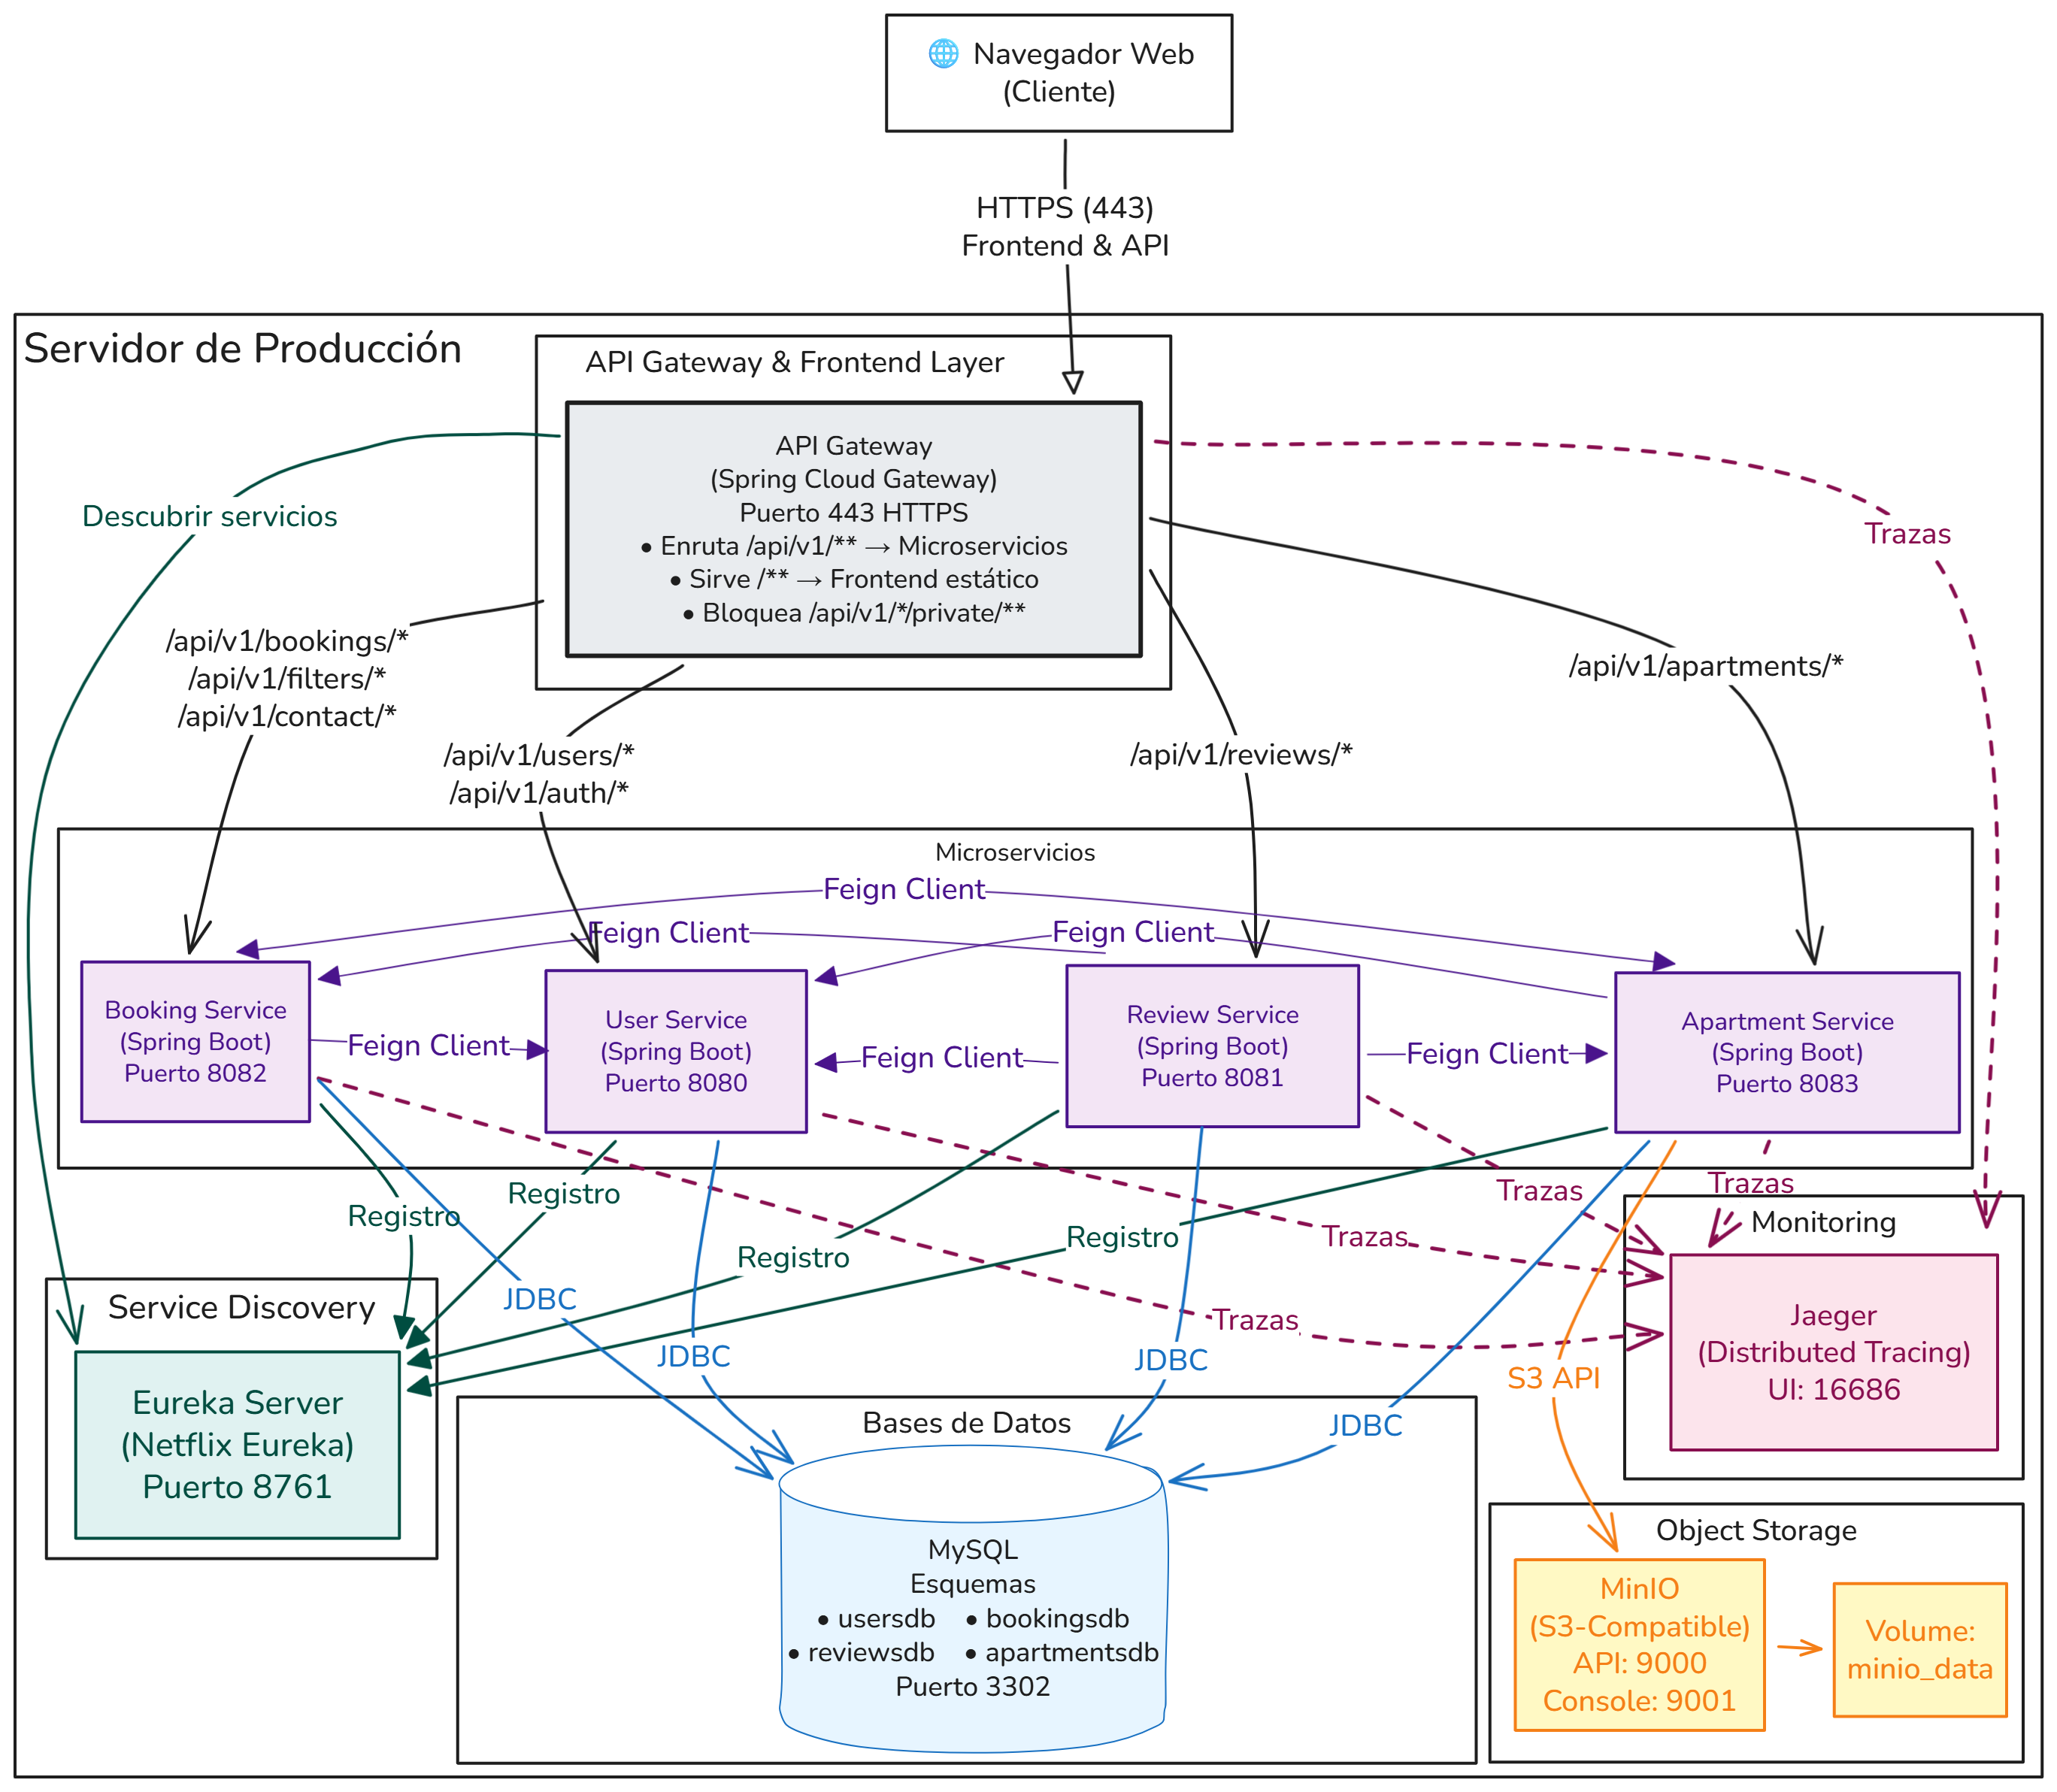
\includegraphics[width=1.2\textwidth, clip=true]{img/deployment_architecture.png}
            \caption{Arquitectura de despliegue: procesos contenerizados, puertos y flujos de comunicación.}
            \label{fig:arquitectura_despliegue}
        \end{figure}

    \subsection{Modelo del Dominio}
        El modelo de dominio representa las entidades principales del sistema, sus atributos clave y las relaciones que definen la lógica del negocio. Debido a la naturaleza distribuida de los microservicios, las relaciones entre dominios distintos no se materializan mediante claves foráneas (\textit{Foreign Keys}) tradicionales en la base de datos, sino a través de referencias lógicas (identificadores) que se validan mediante peticiones REST.

        Las entidades persistentes del sistema son (ver Figura \ref{fig:modelo_dominio}):
        \begin{itemize}
            \item \textbf{User (Usuario):} Representa a los actores del sistema. Contiene atributos como \texttt{id}, \texttt{email} (único), \texttt{password} (encriptada), \texttt{firstName}, \texttt{lastName} y \texttt{role} (USER o ADMIN).
            \item \textbf{Apartment (Apartamento):} Núcleo del catálogo. Sus atributos incluyen \texttt{id}, \texttt{name}, \texttt{description}, \texttt{basePrice}, \texttt{maxGuests}, y una lista de comodidades (\texttt{amenities}) y referencias a imágenes almacenadas en MinIO.
            \item \textbf{Booking (Reserva):} Registra los alquileres. Relaciona un \texttt{userId} y un \texttt{apartmentId}. Incluye \texttt{checkInDate}, \texttt{checkOutDate}, \texttt{totalPrice}, \texttt{status} (CONFIRMED, CANCELLED, COMPLETED) y \texttt{guestCount}.
            \item \textbf{Review (Reseña):} Almacena el \textit{feedback} de los usuarios. Vincula un \texttt{userId} con un \texttt{apartmentId} e incluye \texttt{rating} (1-5), \texttt{comment} y \texttt{createdAt}.
            \item \textbf{Filter (Regla de Precio):} Entidad administrable que define las reglas de precios dinámicos, incluyendo \texttt{name}, \texttt{increment} (booleano), \texttt{value} (porcentaje) y condiciones temporales.
        \end{itemize}

        \begin{figure}[H]
            \centering
            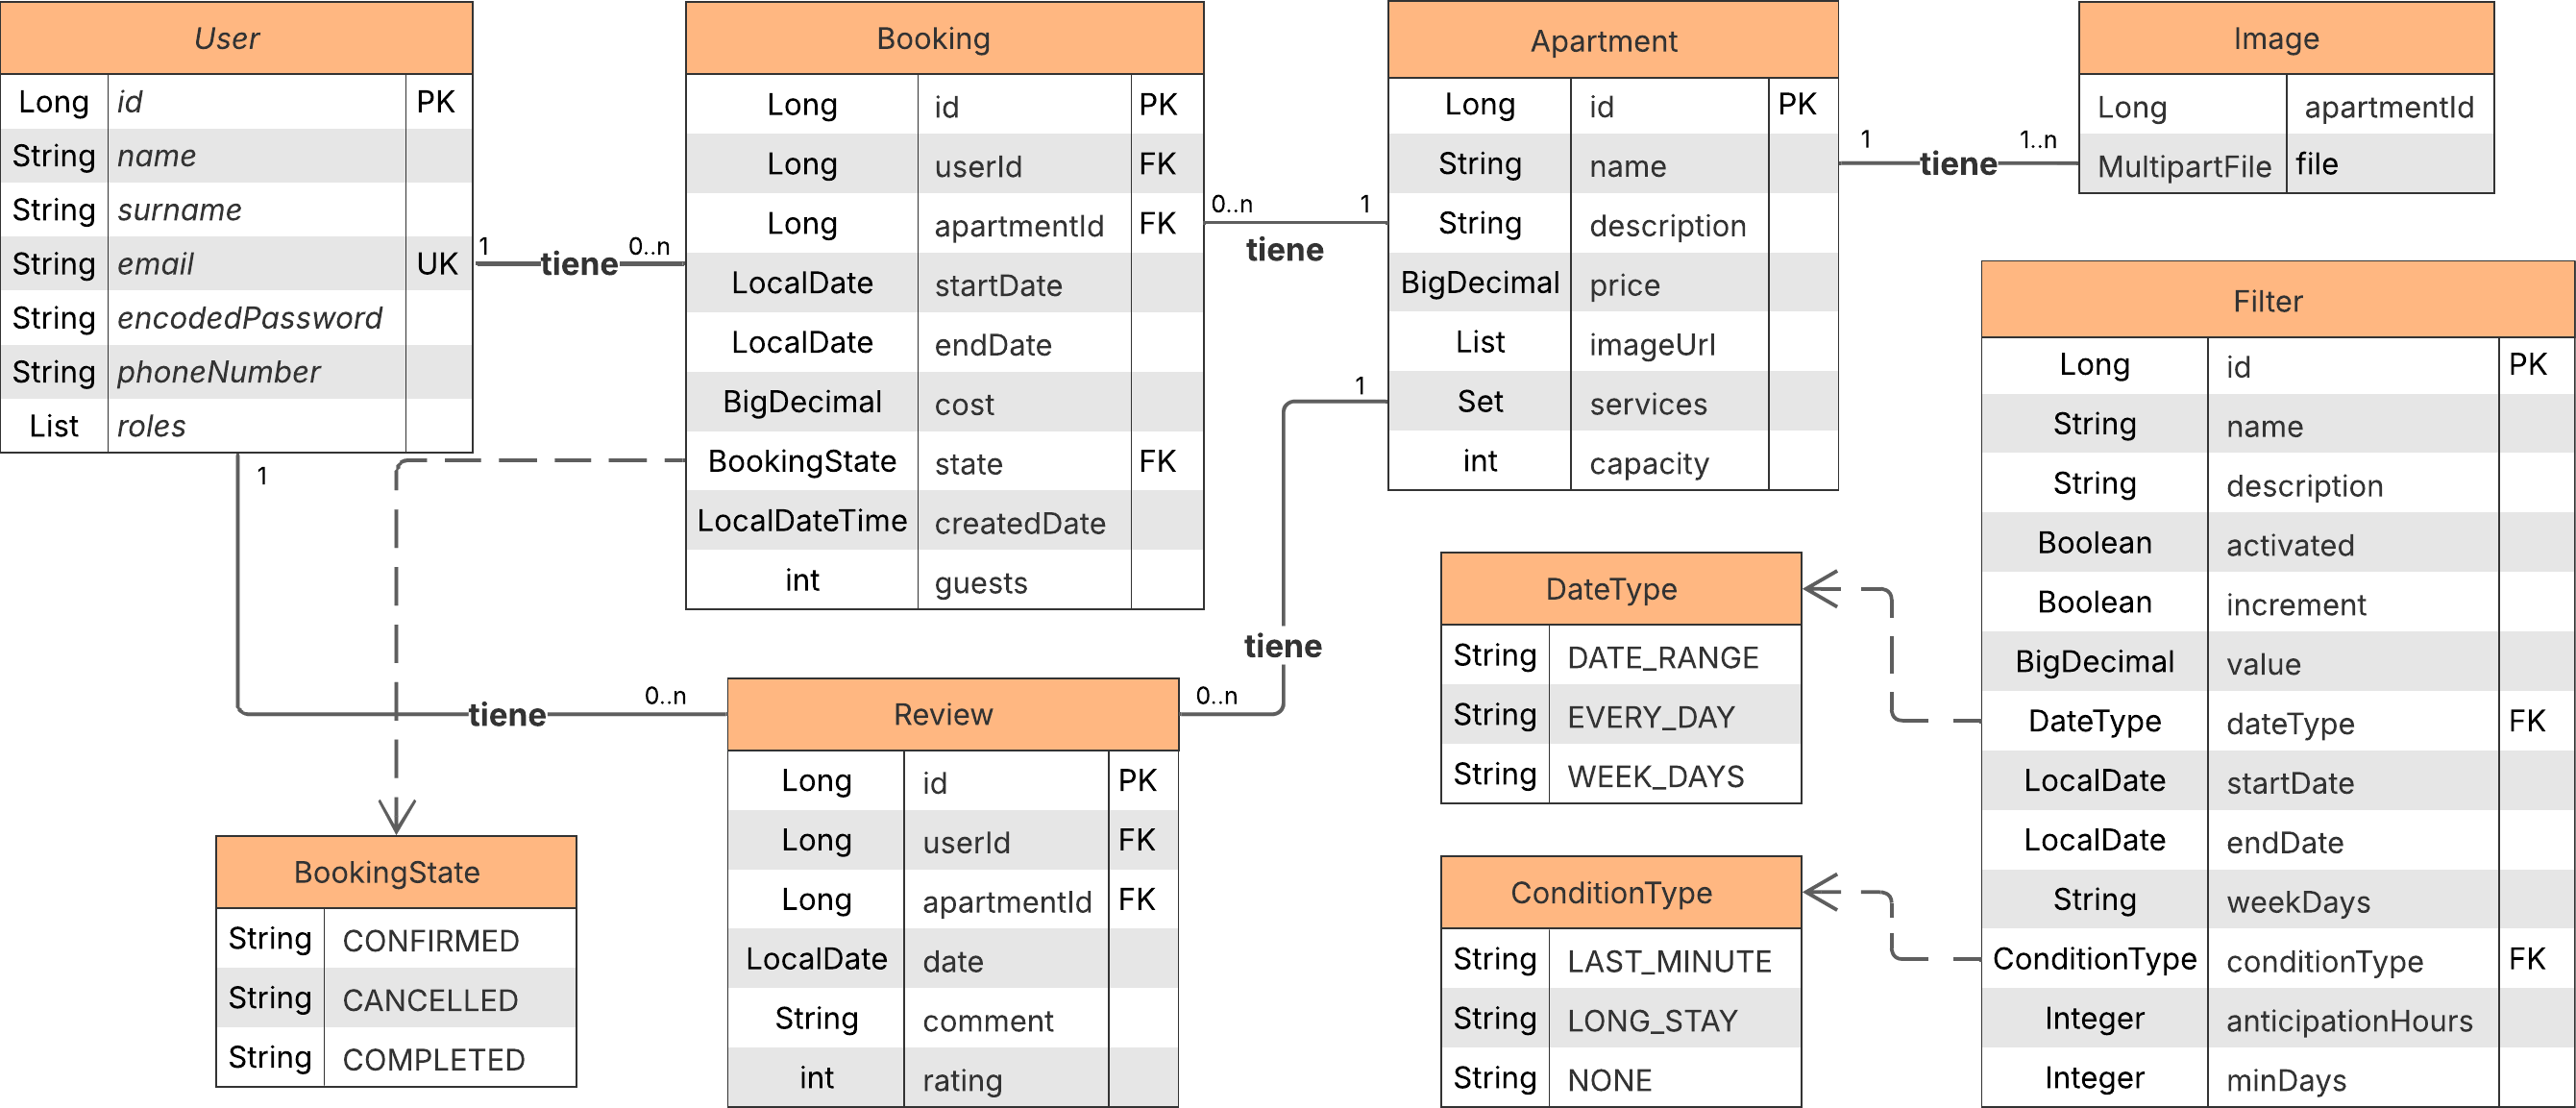
\includegraphics[width=1\textwidth, clip=true]{img/diagrama_entidad.png}
            \caption{Modelo de dominio lógico del sistema Sky Apartments.}
            \label{fig:modelo_dominio}
        \end{figure}

    \subsection{API REST}
        El sistema expone una API RESTful documentada bajo el estándar OpenAPI 3.0. Todas las peticiones del cliente se canalizan a través del \textit{API Gateway} mediante el prefijo \texttt{/api/v1/}. A continuación, se describen a alto nivel los recursos públicos principales, detallando su estructura JSON y las operaciones disponibles agrupadas por método HTTP. Se han omitido de forma deliberada los \textit{endpoints} internos (rutas \texttt{/private/}) diseñados exclusivamente para la comunicación síncrona entre microservicios.

        \subsubsection{Recurso Apartments}
        Gestiona el catálogo de alojamientos, sus características y la comprobación de su disponibilidad.
        \begin{lstlisting}[basicstyle=\jsonbasicfont,frame=single,backgroundcolor=\color{white},rulecolor=\color{black},framerule=0.5pt,numbers=none]
        {
        "id": 1,
        "name": "Ocean View Penthouse",
        "description": "Luxury apartment with panoramic sea views.",
        "price": 150.00,
        "capacity": 4,
        "services": ["WIFI", "TERRACE", "POOL"],
        "imagesUrl": ["https://minio.../image1.jpg"]
        }
        \end{lstlisting}

        \textbf{Operaciones}
        \begin{itemize}
            \item \textbf{GET /api/v1/apartments/} - Obtiene el listado completo paginado de apartamentos.
            \item \textbf{GET /api/v1/apartments/\{id\}} - Obtiene los detalles completos de un apartamento específico.
            \item \textbf{GET /api/v1/apartments/search} - Busca apartamentos filtrando por servicios, capacidad y fechas de disponibilidad.
            \item \textbf{GET /api/v1/apartments/services} - Devuelve el conjunto de todos los servicios/comodidades posibles.
            \item \textbf{GET /api/v1/apartments/\{id\}/availability} - Comprueba si un apartamento está disponible en un rango de fechas.
            \item \textbf{POST /api/v1/apartments} - Crea un nuevo apartamento, soportando subida de imágenes \textit{Multipart} (Requiere rol ADMIN).
            \item \textbf{PUT /api/v1/apartments/\{id\}} - Actualiza la información de un apartamento existente (Requiere rol ADMIN).
            \item \textbf{DELETE /api/v1/apartments/\{id\}} - Elimina un apartamento del catálogo (Requiere rol ADMIN).
        \end{itemize}

    \subsubsection{Recurso Bookings}
        Gestiona el ciclo de vida de las reservas y se encarga del cálculo del precio final basado en fechas.
        \begin{lstlisting}[basicstyle=\jsonbasicfont,frame=single,backgroundcolor=\color{white},rulecolor=\color{black},framerule=0.5pt,numbers=none]
        {
        "id": 1024,
        "userId": 5,
        "apartmentId": 1,
        "startDate": "2026-08-15",
        "endDate": "2026-08-20",
        "guests": 2,
        "cost": 850.50,
        "state": "CONFIRMED",
        "createdDate": "2026-07-01T10:00:00Z"
        }
        \end{lstlisting}

        \textbf{Operaciones}
        \begin{itemize}
            \item \textbf{GET /api/v1/bookings/user/\{userId\}} - Obtiene el historial de reservas paginado de un usuario.
            \item \textbf{GET /api/v1/bookings/apartment/\{apartmentId\}} - Obtiene las reservas asociadas a un apartamento específico.
            \item \textbf{POST /api/v1/bookings} - Crea y confirma una nueva reserva.
            \item \textbf{PUT /api/v1/bookings/\{bookingId\}/dates} - Modifica las fechas de entrada y salida de una reserva existente.
            \item \textbf{DELETE /api/v1/bookings/\{bookingId\}} - Cancela una reserva activa.
        \end{itemize}

    \subsubsection{Recurso Filters}
        Administra el motor de reglas de precios dinámicos aplicables a las reservas.
        \begin{lstlisting}[basicstyle=\jsonbasicfont,frame=single,backgroundcolor=\color{white},rulecolor=\color{black},framerule=0.5pt,numbers=none]
        {
        "id": 1,
        "name": "Weekend Premium",
        "description": "Increment for weekend stays",
        "activated": true,
        "increment": true,
        "value": 15.00,
        "dateType": "WEEK_DAYS",
        "weekDays": "5,6,7",
        "conditionType": "NONE"
        }
        \end{lstlisting}

        \textbf{Operaciones}
        \begin{itemize}
            \item \textbf{GET /api/v1/filters} - Obtiene el listado paginado de todas las reglas configuradas.
            \item \textbf{GET /api/v1/filters/applicable} - Calcula y devuelve qué reglas de precio aplicarían para un rango de fechas concreto.
            \item \textbf{POST /api/v1/filters} - Crea una nueva regla de precios dinámica (Requiere rol ADMIN).
            \item \textbf{PUT /api/v1/filters/\{id\}} - Modifica la configuración de una regla existente (Requiere rol ADMIN).
            \item \textbf{DELETE /api/v1/filters/\{id\}} - Elimina una regla del sistema (Requiere rol ADMIN).
        \end{itemize}

    \subsubsection{Recurso Users y Auth}
        Gestiona la identidad de los clientes, sus perfiles y el proceso de autenticación.
        \begin{lstlisting}[basicstyle=\jsonbasicfont,frame=single,backgroundcolor=\color{white},rulecolor=\color{black},framerule=0.5pt,numbers=none]
        {
        "id": 5,
        "name": "Carlos",
        "surname": "García",
        "email": "cliente@example.com",
        "phoneNumber": "600000000",
        "roles": ["ROLE_USER"]
        }
        \end{lstlisting}

        \textbf{Operaciones de Usuario}
        \begin{itemize}
            \item \textbf{GET /api/v1/users/me} - Obtiene el perfil completo del usuario autenticado actual.
            \item \textbf{GET /api/v1/users/\{id\}} - Obtiene un usuario específico por su ID.
            \item \textbf{POST /api/v1/users} - Registra un nuevo usuario en el sistema.
            \item \textbf{PUT /api/v1/users/\{id\}} - Actualiza la información personal de un usuario.
            \item \textbf{DELETE /api/v1/users/\{id\}} - Elimina a un usuario del sistema.
        \end{itemize}

        \textbf{Operaciones de Autenticación}
        \begin{itemize}
            \item \textbf{POST /api/v1/auth/login} - Valida credenciales y emite las cookies seguras con los \textit{Auth} y \textit{Refresh tokens}.
            \item \textbf{POST /api/v1/auth/refresh} - Renueva el \textit{token} de acceso caducado utilizando el \textit{Refresh token} de la cookie.
            \item \textbf{POST /api/v1/auth/logout} - Invalida la sesión actual y limpia las cookies del navegador.
        \end{itemize}

    \subsubsection{Recurso Reviews}
        Centraliza el sistema de valoraciones y \textit{feedback} de los huéspedes.
        \begin{lstlisting}[basicstyle=\jsonbasicfont,frame=single,backgroundcolor=\color{white},rulecolor=\color{black},framerule=0.5pt,numbers=none]
        {
        "id": 42,
        "userId": 5,
        "userName": "Carlos G.",
        "apartmentId": 1,
        "date": "2026-08-21",
        "comment": "Estancia inolvidable, todo impecable.",
        "rating": 5
        }
        \end{lstlisting}

        \textbf{Operaciones}
        \begin{itemize}
            \item \textbf{GET /api/v1/reviews/apartment/\{apartmentId\}} - Obtiene la lista paginada de reseñas publicadas en un apartamento.
            \item \textbf{GET /api/v1/reviews/apartment/\{apartmentId\}/rating} - Calcula y devuelve la nota media global de un apartamento.
            \item \textbf{GET /api/v1/reviews/can-review} - Verifica si un usuario concreto está autorizado para dejar una reseña (requiere estancia completada).
            \item \textbf{POST /api/v1/reviews} - Publica una nueva reseña en un apartamento.
            \item \textbf{PUT /api/v1/reviews/\{reviewId\}} - Edita el texto y la valoración de una reseña existente.
            \item \textbf{DELETE /api/v1/reviews/\{reviewId\}} - Elimina una reseña publicada.
        \end{itemize}

    \subsubsection{Recurso Contact}
        Punto de entrada para consultas públicas o dudas comerciales.
        \begin{lstlisting}[basicstyle=\jsonbasicfont,frame=single,backgroundcolor=\color{white},rulecolor=\color{black},framerule=0.5pt,numbers=none]
        {
        "name": "Ana Martínez",
        "email": "ana.mtz@example.com",
        "subject": "Duda sobre accesibilidad",
        "message": "¿El apartamento dispone de rampa en el portal?"
        }
        \end{lstlisting}

        \textbf{Operaciones}
        \begin{itemize}
            \item \textbf{POST /api/v1/contact} - Envía un mensaje desde el formulario de contacto público hacia el administrador mediante integración con el servicio de correo electrónico.
        \end{itemize}

    \subsection{Arquitectura del Servidor}
        Para garantizar la separación de responsabilidades y la mantenibilidad del código, cada uno de los microservicios Spring Boot sigue internamente un patrón de arquitectura en capas (Layered Architecture) \cite[pp.~20--24]{buschmann1996} (ver Figura \ref{fig:arquitectura_servidor}).

        \begin{figure}[H]
            \centering
            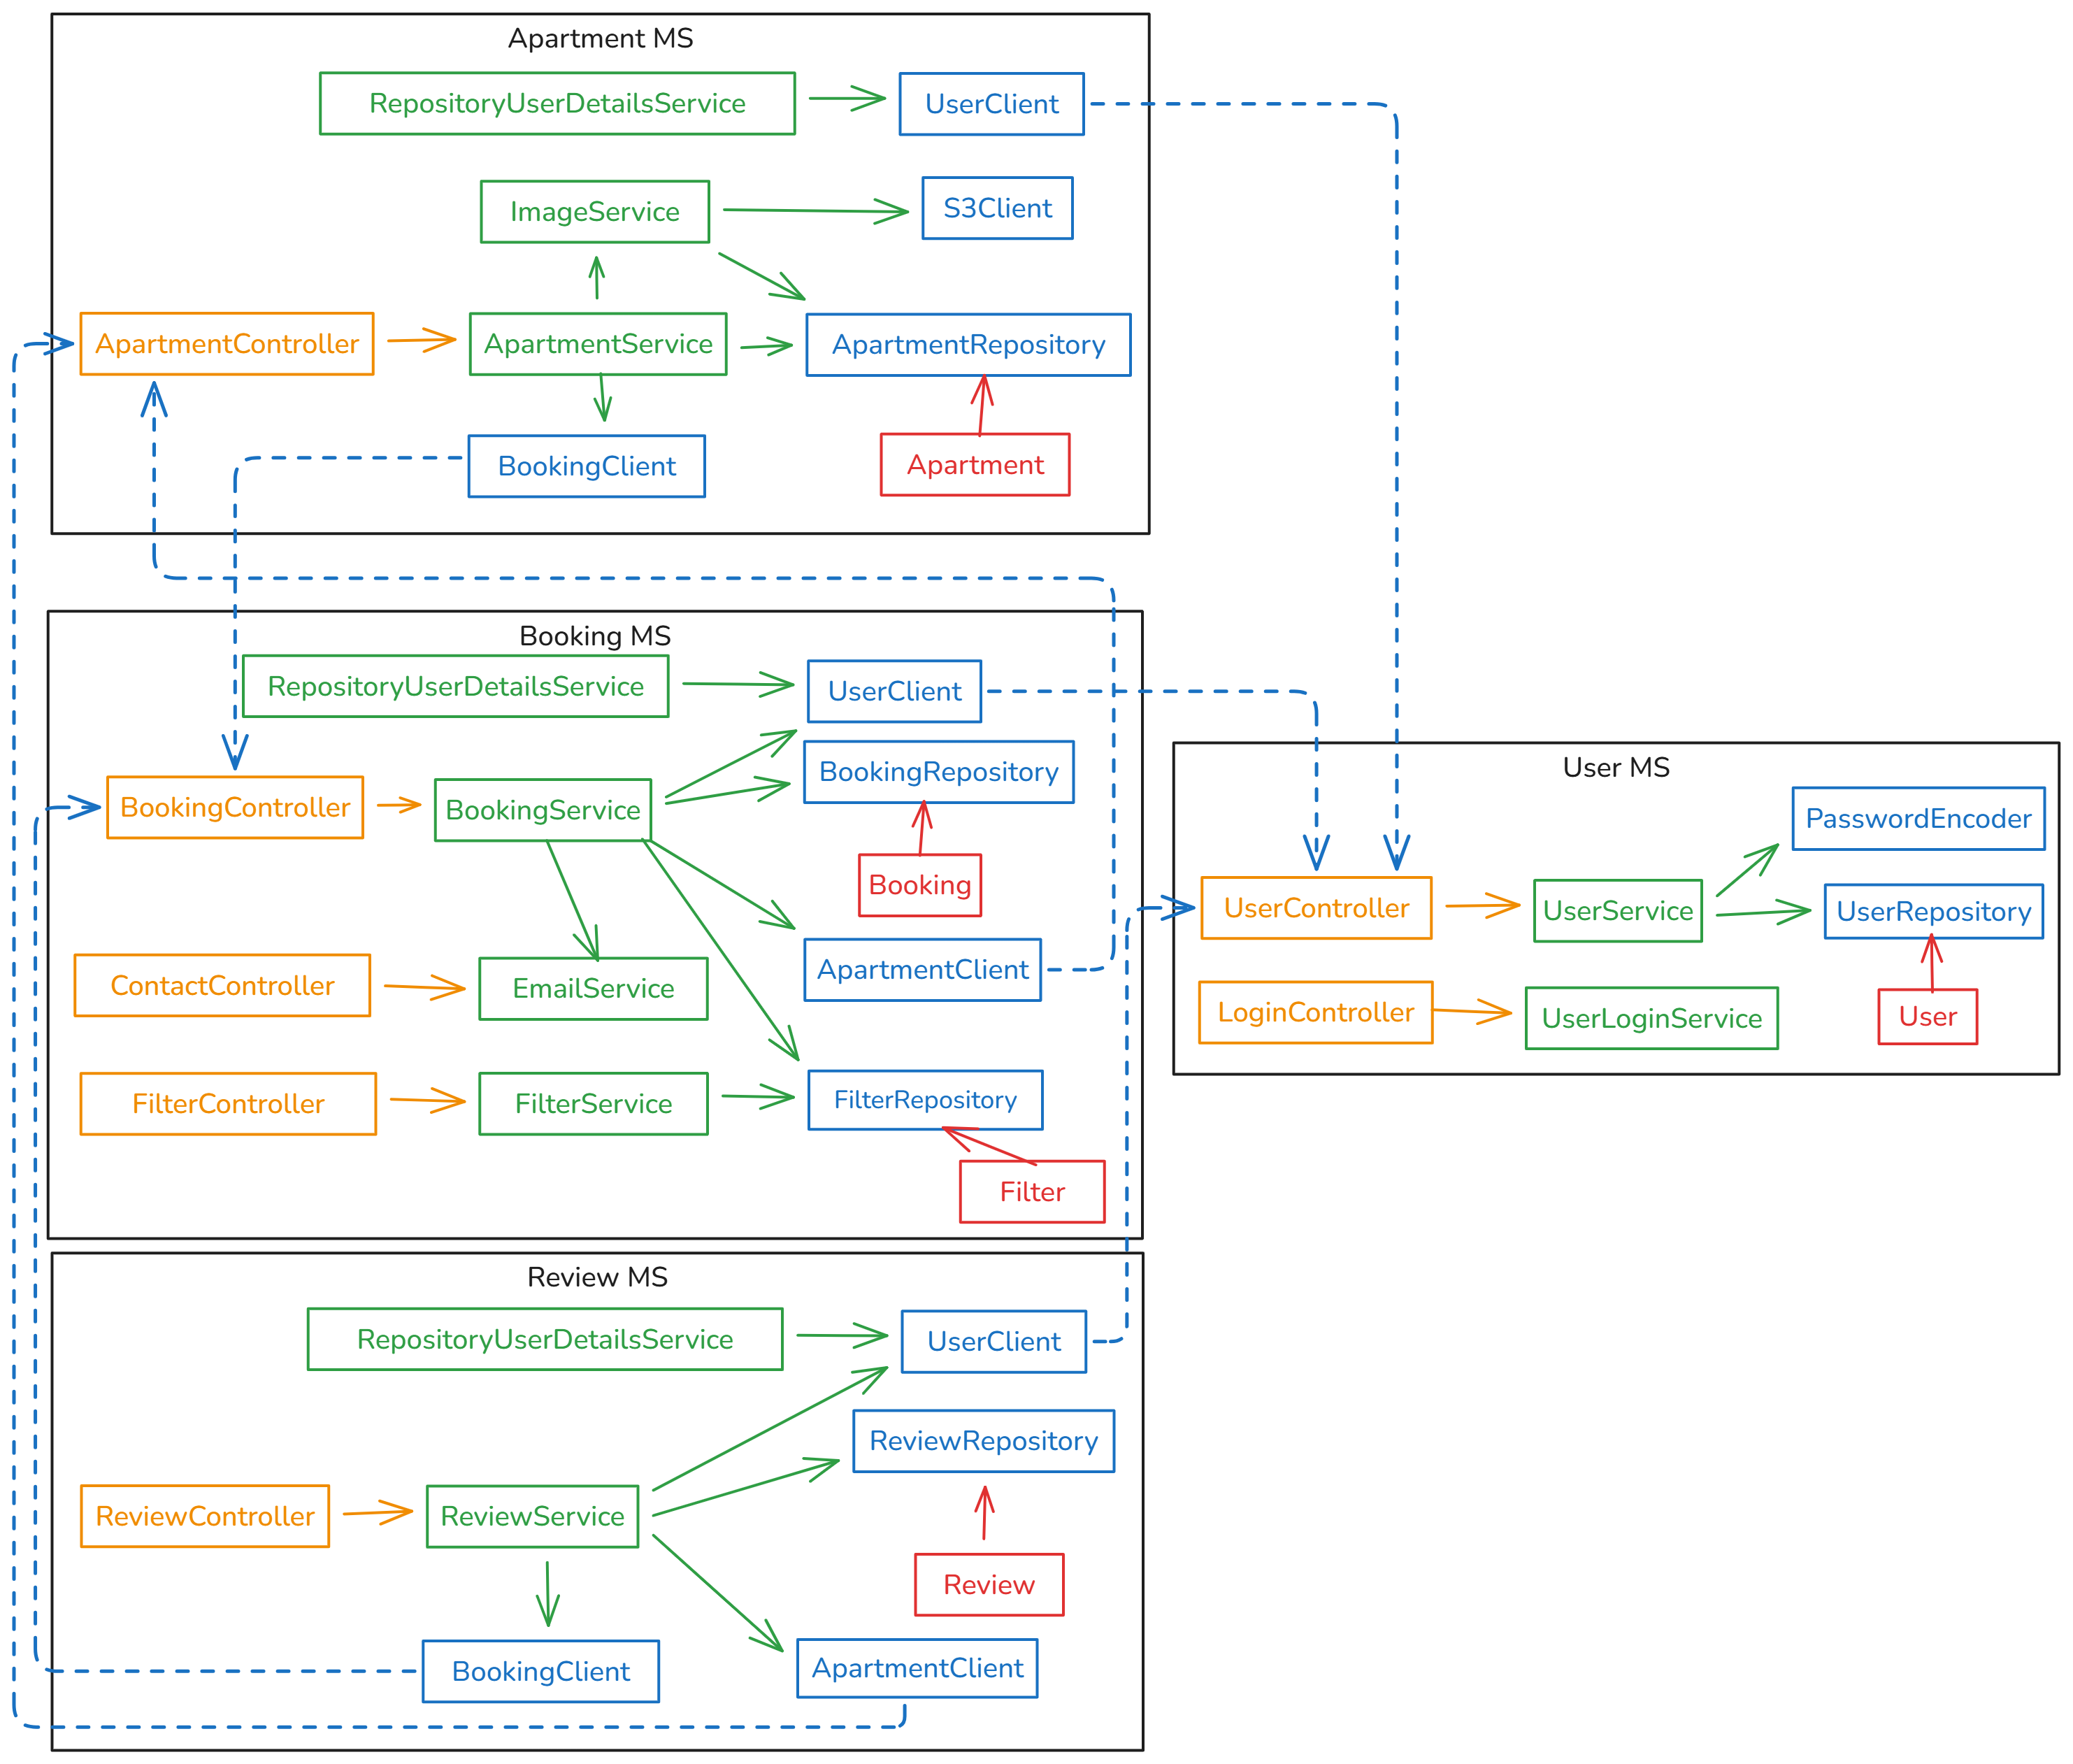
\includegraphics[width=1\textwidth, clip=true]{img/diagrama_server.png}
            \caption{Arquitectura en capas del servidor backend y comunicación entre microservicios.}
            \label{fig:arquitectura_servidor}
        \end{figure}

        Las responsabilidades de cada capa son las siguientes:
        \begin{itemize}
            \item \textbf{Controladores (\textit{Controllers}):} Capa externa que recibe las peticiones HTTP REST, valida los datos de entrada mediante el patrón DTO \cite[pp.~401--402]{fowler2002} y devuelve las respuestas con los códigos de estado adecuados, delegando siempre la lógica de negocio.
            \item \textbf{Servicios (\textit{Services}):} Núcleo del microservicio. Concentran toda la lógica de negocio, los cálculos algorítmicos (ej. motor de precios) y orquestan la comunicación síncrona con otros servicios mediante \textit{Feign Clients}.
            \item \textbf{Repositorios (\textit{Repositories}):} Abstraen el acceso a la base de datos implementando el patrón Repositorio \cite[pp.~322--327]{fowler2002} mediante Spring Data JPA, permitiendo realizar operaciones CRUD y consultas personalizadas sin necesidad de escribir sentencias SQL explícitas.
            \item \textbf{Entidades (\textit{Entities}):} Clases Java que representan el modelo de dominio y se mapean directamente a las tablas de MySQL mediante anotaciones de Hibernate.
        \end{itemize}

    \subsection{Arquitectura del Cliente}
        El cliente web construido con Angular sigue una arquitectura modular basada en componentes, diseñada para fomentar la reutilización de código y la reactividad de la interfaz de usuario (ver Figura \ref{fig:arquitectura_cliente}).

        \begin{figure}[H]
            \centering
            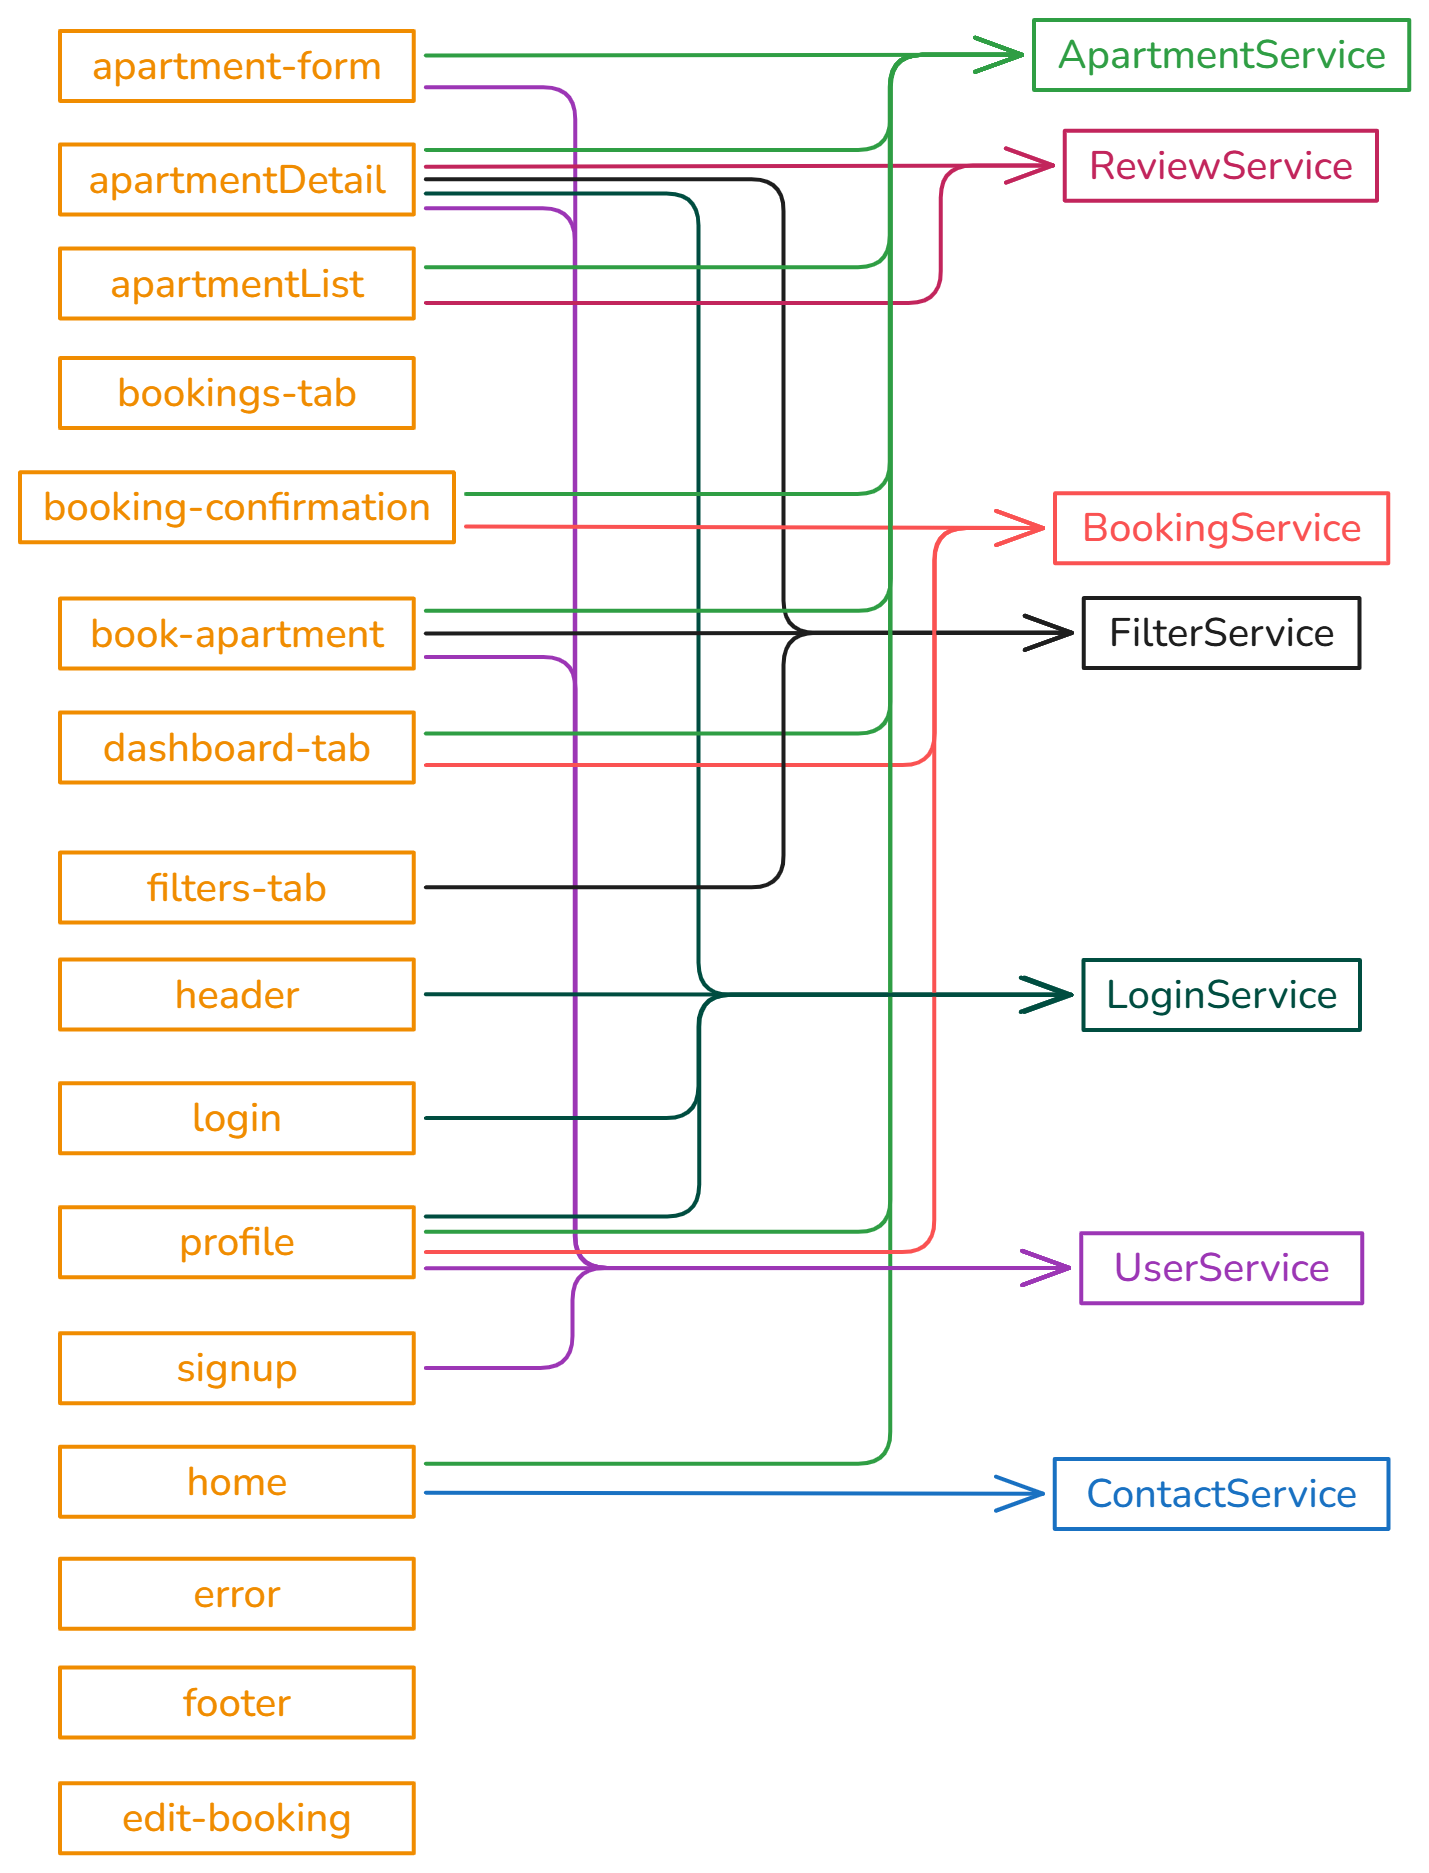
\includegraphics[width=0.6\textwidth, clip=true]{img/diagrama_cliente.png}
            \caption{Arquitectura del cliente Angular: Componentes, Servicios e Interceptores.}
            \label{fig:arquitectura_cliente}
        \end{figure}

        La separación por responsabilidades en el frontend se estructura en las siguientes capas:
        \begin{itemize}
            \item \textbf{Componentes (\textit{Components}):} Gestionan la vista (HTML/CSS) y la interacción del usuario. Se dividen en componentes de enrutamiento (páginas completas) y componentes presentacionales reutilizables (ej. \textit{Navbar} o \textit{Cards}).
            \item \textbf{Servicios (\textit{Services}):} Clases que aplican el patrón de inyección de dependencias \cite{fowler2004} para centralizar la lógica de negocio y aislar la comunicación externa mediante \texttt{HttpClient}. Destaca el uso de RxJS (\textit{BehaviorSubjects}) para gestionar estados globales, como la autenticación en el \textit{AuthService}.
            \item \textbf{Interceptores (\textit{Interceptors}):} \textit{Middleware} HTTP que procesa peticiones salientes y respuestas entrantes. Son fundamentales para aplicar lógicas globales de forma transparente, como ejecutar el refresco silencioso de tokens (\textit{Silent Refresh}) al detectar errores 401.
        \end{itemize}
\section{Implementación} 
\label{sec:implementacion}

En esta sección se describen los aspectos más relevantes del proceso de construcción del software, destacando decisiones de diseño significativas, desafíos técnicos encontrados y las soluciones algorítmicas adoptadas. Se focaliza la atención en aquellos componentes de la lógica de negocio que requirieron un mayor nivel de abstracción y estudio durante el desarrollo.

\subsection{Gestión de Autenticación y Seguridad con JWT}
Uno de los retos técnicos iniciales del sistema fue implementar un mecanismo de autenticación robusto, seguro y transparente para el usuario en una arquitectura distribuida sin estado (\textit{stateless}). La solución adoptada utiliza \textit{JSON Web Tokens} (JWT) combinada con una estrategia de \textit{Silent Refresh} gestionada por cookies de tipo \textit{HttpOnly}.

\subsubsection{Arquitectura de Seguridad y Flujo de Autenticación}
El sistema delega la responsabilidad de la seguridad de forma híbrida: el \textbf{User Service} actúa como servidor central de autorización, mientras que el resto de los microservicios actúan como recursos protegidos que validan la identidad de forma descentralizada.

Como se detalla en la Figura~\ref{fig:diagrama_jwt}, el flujo de autenticación garantiza que las credenciales sensibles y los tokens nunca persistan en el almacenamiento local del cliente (como \textit{LocalStorage}), utilizando el navegador como almacén seguro mediante cookies.

\begin{figure}[h]
    \centering
    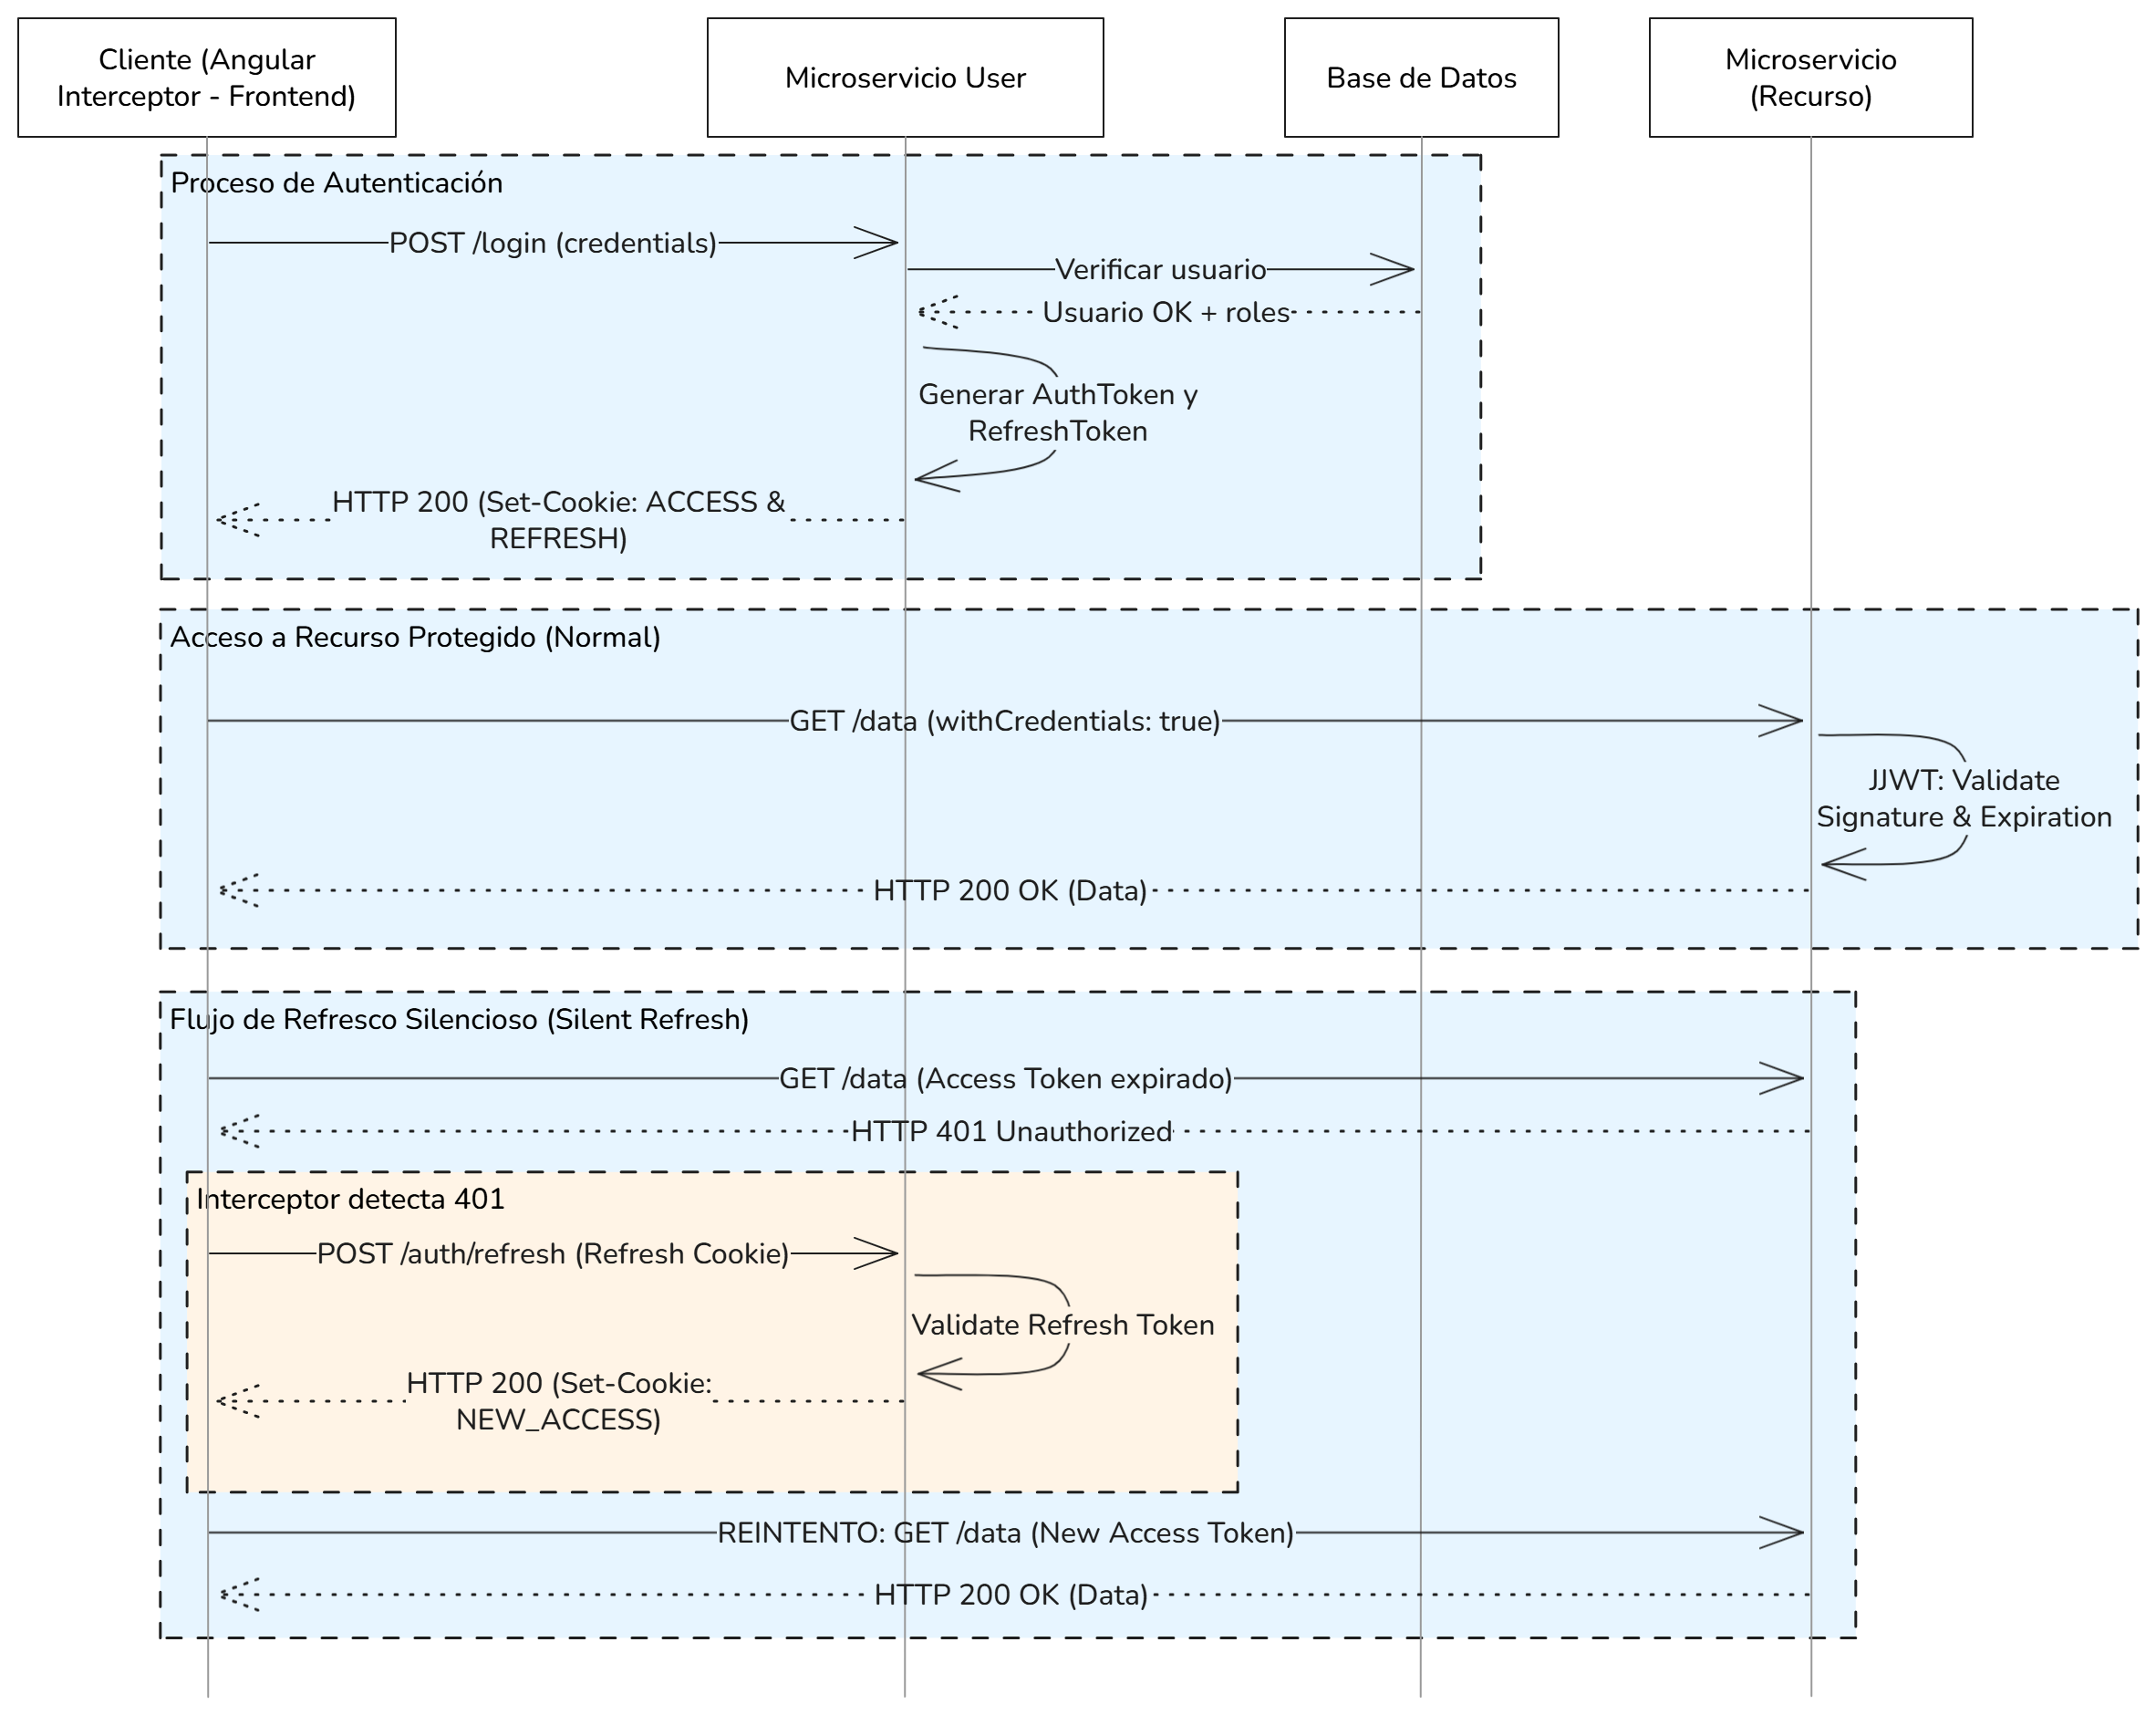
\includegraphics[width=0.9\textwidth]{img/diagrama_jwt.png}
    \caption{Diagrama de secuencia del proceso de autenticación, validación y refresco de tokens.}
    \label{fig:diagrama_jwt}
\end{figure}

\subsubsection{Generación de Tokens y Persistencia}
Tras la validación de credenciales mediante el \texttt{AuthenticationManager} de Spring Security, el sistema genera dos tipos de tokens con la librería JJWT (ver Código~\ref{lst:login_logic}):
\begin{itemize}
    \item \textbf{Auth Token}: Token de acceso de corta duración (5 minutos) firmado con el algoritmo HMAC-SHA512.
    \item \textbf{Refresh Token}: Token de larga duración (7 días) utilizado exclusivamente para solicitar nuevos tokens de acceso al servidor.
\end{itemize}

Ambos tokens se envían al cliente mediante el encabezado HTTP \texttt{Set-Cookie}, configurados estrictamente como \textit{HttpOnly} para mitigar los ataques de inyección de código (\textit{Cross-Site Scripting} o XSS), ya que impiden que el código JavaScript del cliente acceda a ellos.

\begin{lstlisting}[language=Java, caption={Lógica de login y creación de cookies en el User Service}, label={lst:login_logic}]
public ResponseEntity<AuthResponse> login(HttpServletResponse response, LoginRequest loginRequest) {
    Authentication auth = authenticationManager.authenticate(
        new UsernamePasswordAuthenticationToken(loginRequest.getUsername(), loginRequest.getPassword()));
    
    UserDetails user = (UserDetails) auth.getPrincipal();
    
    // Generacion de tokens y persistencia en cookies HttpOnly
    response.addCookie(buildTokenCookie(TokenType.ACCESS, jwtProvider.generateAccessToken(user)));
    response.addCookie(buildTokenCookie(TokenType.REFRESH, jwtProvider.generateRefreshToken(user)));

    return ResponseEntity.ok(new AuthResponse(Status.SUCCESS, "Auth successful"));
}
\end{lstlisting}

\subsubsection{Validación y Refresco Silencioso (Silent Refresh)}
Un aspecto diferencial de la implementación radica en la gestión de caducidad desde el \textbf{Interceptor HTTP de Angular}. Dado que el \textit{Auth Token} tiene una vida muy corta por motivos de seguridad, el interceptor monitoriza todas las respuestas del servidor. 

Si un microservicio devuelve un código de error \texttt{401 Unauthorized}, el interceptor de Angular captura el error, pausa temporalmente las peticiones salientes y lanza una petición asíncrona al \textit{endpoint} \texttt{/auth/refresh}. Si el \textit{Refresh Token} es válido, el servidor emite una nueva cookie y el interceptor reintenta la operación original automáticamente, sin que la experiencia del usuario se vea interrumpida.

\subsubsection{Seguridad de las Claves}
Para garantizar la integridad del sistema en diferentes entornos, la clave secreta JWT no se encuentra codificada en el código fuente (\textit{hardcoded}). Se gestiona mediante variables de entorno inyectadas en tiempo de ejecución, lo que permite rotar las claves en producción sin necesidad de recompilar los artefactos.

\subsection{Motor de Precios Dinámicos}
La funcionalidad troncal y más compleja de la lógica de negocio ha sido el \textbf{motor de precios dinámico}, que permite ajustar el coste por noche de los alojamientos en tiempo real basándose en reglas contextuales.

\subsubsection{Concepto y Arquitectura}
Un filtro de precio es una regla que especifica el tipo de ajuste (incremento o descuento), el porcentaje de ajuste y las condiciones de aplicación.

\subsubsection{Diseño Flexible de la Entidad Filter}
El aspecto más destacable del sistema es el diseño de la entidad \texttt{Filter}, que utiliza un patrón de configuración flexible mediante campos opcionales que se combinan para representar diferentes tipos de reglas (\ref{lst:filter}):

\begin{lstlisting}[ caption={Entidad Filter para sistema dinámico de precios}, label={lst:filter}]
@Entity
public class Filter {
    private Long id;
    private String name;
    private String description;
    private Boolean activated;
    private Boolean increment;        // true = incremento, false = descuento
    private BigDecimal value;         // Porcentaje de ajuste
    
    // Configuracion temporal
    private DateType dateType;        // DATE_RANGE | EVERY_DAY | WEEK_DAYS | DATE_RANGE_WEEK_DAYS
    private LocalDate startDate;      // Requerido si dateType incluye rango
    private LocalDate endDate;        // Requerido si dateType incluye rango
    private String weekDays;          // Requerido si dateType incluye dias (valores: 1-7)
    
    // Condiciones adicionales
    private ConditionType conditionType;  // LAST_MINUTE | LONG_STAY | NONE
    private Integer anticipationHours;    // Requerido si conditionType = LAST_MINUTE
    private Integer minDays;              // Requerido si conditionType = LONG_STAY
}
\end{lstlisting}












La clave del diseño está en que los campos obligatorios dependen de los valores de los enums. El sistema utiliza dos enums:

\textbf{DateType} determina cuándo aplica el filtro temporalmente:
\begin{itemize}
\item \texttt{DATE\_RANGE}: Aplica en un rango específico de fechas (requiere \texttt{startDate} y \texttt{endDate})
\item \texttt{WEEK\_DAYS}: Aplica solo ciertos días de la semana (requiere \texttt{weekDays})
\item \texttt{EVERY\_DAY}: Aplica todos los días sin restricción
\item \texttt{DATE\_RANGE\_WEEK\_DAYS}: Aplica ciertos días dentro de un rango

(requiere \texttt{startDate}, \texttt{endDate} y \texttt{weekDays})
\end{itemize}

\textbf{ConditionType} añade condiciones adicionales sobre la reserva:
\begin{itemize}
\item \texttt{LAST\_MINUTE}: Aplica para reservas con poca antelación

(requiere \texttt{anticipationHours})
\item \texttt{LONG\_STAY}: Aplica solo para estancias de duración mínima (requiere \texttt{minDays})
\item \texttt{NONE}: Sin condición adicional
\end{itemize}

Este enfoque proporciona máxima flexibilidad porque permite combinaciones complejas (por ejemplo, descuento solo en verano y solo para estancias largas), utiliza validación condicional de campos según los enums seleccionados, presenta una interfaz adaptativa que muestra/oculta campos dinámicamente y evita la proliferación de entidades.

Con esta estructura, el sistema puede representar cualquier combinación lógica de restricciones temporales y condiciones de reserva, cubriendo escenarios desde descuentos generales permanentes hasta combinaciones complejas como estancias largas en fines de semana de verano. Esto representa múltiples tipos diferentes de reglas de negocio sin necesidad de crear múltiples entidades o tablas.

Esta arquitectura de \textbf{configuración sobre código} es un ejemplo de aplicación del principio de diseño ``Open/Closed'': el sistema está abierto a extensión (se pueden crear infinitas combinaciones de reglas) pero cerrado a modificación (no hay que cambiar código para añadir nuevos tipos de reglas).

\subsubsection{Consulta de Filtros Aplicables}
El sistema expone un endpoint que permite consultar qué filtros aplicarían a unas fechas específicas antes de realizar la reserva:

\texttt{GET \\ /api/v1/filters/applicable?checkIn=2026-07-16\&checkOut=2026-07-18}

La respuesta organiza los filtros por fecha, mostrando para cada noche de la estancia qué ajustes de precio aplican:
 \begin{lstlisting}
    {
        "checkInDate": "2026-07-16",
        "checkOutDate": "2026-07-18",
        "totalNights": 2,
        "filtersByDate": {
            "2026-07-16": [],
            "2026-07-17": [
                {
                    "id": 1,
                    "name": "Weekend Premium",
                    "description": "Price increase for Friday, Saturday and Sunday nights",
                    "activated": true,
                    "increment": true,
                    "value": 20.00,
                    "dateType": "WEEK_DAYS",
                    "startDate": null,
                    "endDate": null,
                    "weekDays": "5,6,7",
                    "conditionType": "NONE",
                    "anticipationHours": null,
                    "minDays": null,
                    "createdAt": null,
                    "updatedAt": null
                }
            ]
        }
    }
 \end{lstlisting}
 
Esta estructura permite al frontend mostrar una previsualización del precio desglosado noche por noche, dando transparencia al usuario sobre cómo se ha calculado el precio total.


\subsubsection{Cálculo del Precio Final}
Cuando se crea una reserva, el Booking Service obtiene el precio base del apartamento, consulta los filtros aplicables y, para cada noche, aplica secuencialmente cada filtro activo sobre el precio base, acumulando el precio ajustado al total.

Por ejemplo, si un apartamento cuesta \EUR{100}/noche y el usuario reserva un viernes con 20\% de incremento por fin de semana más 10\% de descuento por reserva anticipada, el precio final de esa noche sería \EUR{110} (\EUR{100} + \EUR{20} - \EUR{10}).

\subsubsection{Ventajas del Sistema}
Este diseño proporciona:
\begin{itemize}
\item \textbf{Flexibilidad total}: Los administradores pueden crear cualquier combinación de reglas sin modificar código ni base de datos
\item \textbf{Transparencia}: Los usuarios ven exactamente qué ajustes se están aplicando y por qué
\item \textbf{Competitividad}: Permite implementar estrategias de pricing dinámico similares al \textit{yield management}\footnote{Yield management: estrategia de gestión de ingresos que ajusta precios según demanda y disponibilidad \cite{kimes1989}.} utilizado por aerolíneas y hoteles
\item \textbf{Automatización}: Los precios se ajustan automáticamente según las reglas configuradas, sin intervención manual
\item \textbf{Experimentación}: Fácil probar diferentes estrategias activando/desactivando filtros y midiendo su impacto
\item \textbf{Escalabilidad}: El sistema puede manejar decenas de filtros simultáneos sin degradación de rendimiento
\end{itemize}
Los administradores gestionan los filtros desde un panel dedicado en el frontend, donde pueden crear, editar, activar/desactivar y eliminar reglas mediante formularios intuitivos, sin necesidad de conocimientos técnicos ni programación.

\subsection{Envío de Emails con JavaMailSender}
El Booking Service implementa funcionalidad de notificaciones por email usando Spring Mail.

\subsubsection{Configuración del Servidor SMTP}
La configuración utiliza Gmail SMTP\footnote{SMTP: Simple Mail Transfer Protocol, protocolo estándar para envío de correo electrónico} con autenticación de dos factores mediante contraseña de aplicación. Las credenciales se externalizan mediante variables de entorno para diferentes entornos, permitiendo flexibilidad entre desarrollo y producción.

\subsubsection{Servicio de Email}
El \texttt{EmailService} encapsula la lógica de envío utilizando \texttt{JavaMailSender} y \texttt{MimeMessage} para permitir HTML y archivos adjuntos, con soporte UTF-8 para caracteres internacionales. El servicio implementa manejo de errores silencioso: un fallo en el email no impide crear la reserva.

El servicio proporciona múltiples tipos de notificaciones: confirmación al crear una reserva, actualización al modificar, cancelación y recordatorio programado antes del check-in.


\section{Control de calidad} 
\label{sec:control_calidad}

La estrategia de pruebas del proyecto abarca múltiples niveles tanto en el backend como en el frontend, garantizando la calidad, fiabilidad y correcto funcionamiento del sistema mediante pruebas automatizadas que cubren desde la validación de componentes individuales hasta la verificación de flujos completos de usuario.

\subsection{Estrategia de Testing}
El proyecto sigue la pirámide de testing clásica \cite{fowler2012}, distribuyendo las pruebas en tres niveles:
\begin{itemize}
\item \textbf{Base - Tests Unitarios}: Mayor cantidad de pruebas, ejecución rápida, validan componentes aislados
\item \textbf{Medio - Tests de Integración}: Cantidad moderada, verifican interacciones entre componentes y con infraestructura real
\item \textbf{Cima - Tests End-to-End}: Menor cantidad, costosos pero verifican flujos completos de usuario
\end{itemize}

Esta distribución permite detectar fallos rápidamente en las fases tempranas del desarrollo mientras se garantiza que el sistema funciona correctamente como un todo.

\subsection{Pruebas del Backend}
Los microservicios del backend han sido sometidos a tres tipos de pruebas automatizadas para garantizar la corrección de la lógica de negocio, la persistencia de datos y la comunicación entre servicios.

\subsubsection{Tipos de Pruebas Implementadas}
\begin{itemize}
    \item \textbf{Tests Unitarios:} Validan la lógica de negocio de forma aislada utilizando Mockito para simular dependencias (repositorios y clientes Feign), sin requerir el levantamiento de bases de datos o servicios externos.
    \item \textbf{Tests de Integración:} Verifican el comportamiento del sistema con bases de datos reales mediante contenedores MySQL efímeros (Testcontainers). Validan el mapeo de entidades JPA, las consultas personalizadas y la integridad transaccional.
    \item \textbf{Tests End-to-End (E2E):} Validan flujos completos a través del \textit{API Gateway} realizando peticiones HTTP reales con REST Assured. Verifican la autenticación JWT y la correcta comunicación cruzada entre los distintos microservicios en ejecución.
\end{itemize}

\subsubsection{Cobertura de Código por Microservicio}
La cobertura se mide mediante JaCoCo, que genera reportes HTML detallados tras ejecutar \texttt{mvn test}. Las Figuras \ref{fig:jacoco_apartment}, \ref{fig:jacoco_user}, \ref{fig:jacoco_booking} y \ref{fig:jacoco_review} muestran los reportes.

\begin{figure}[H]
\centering
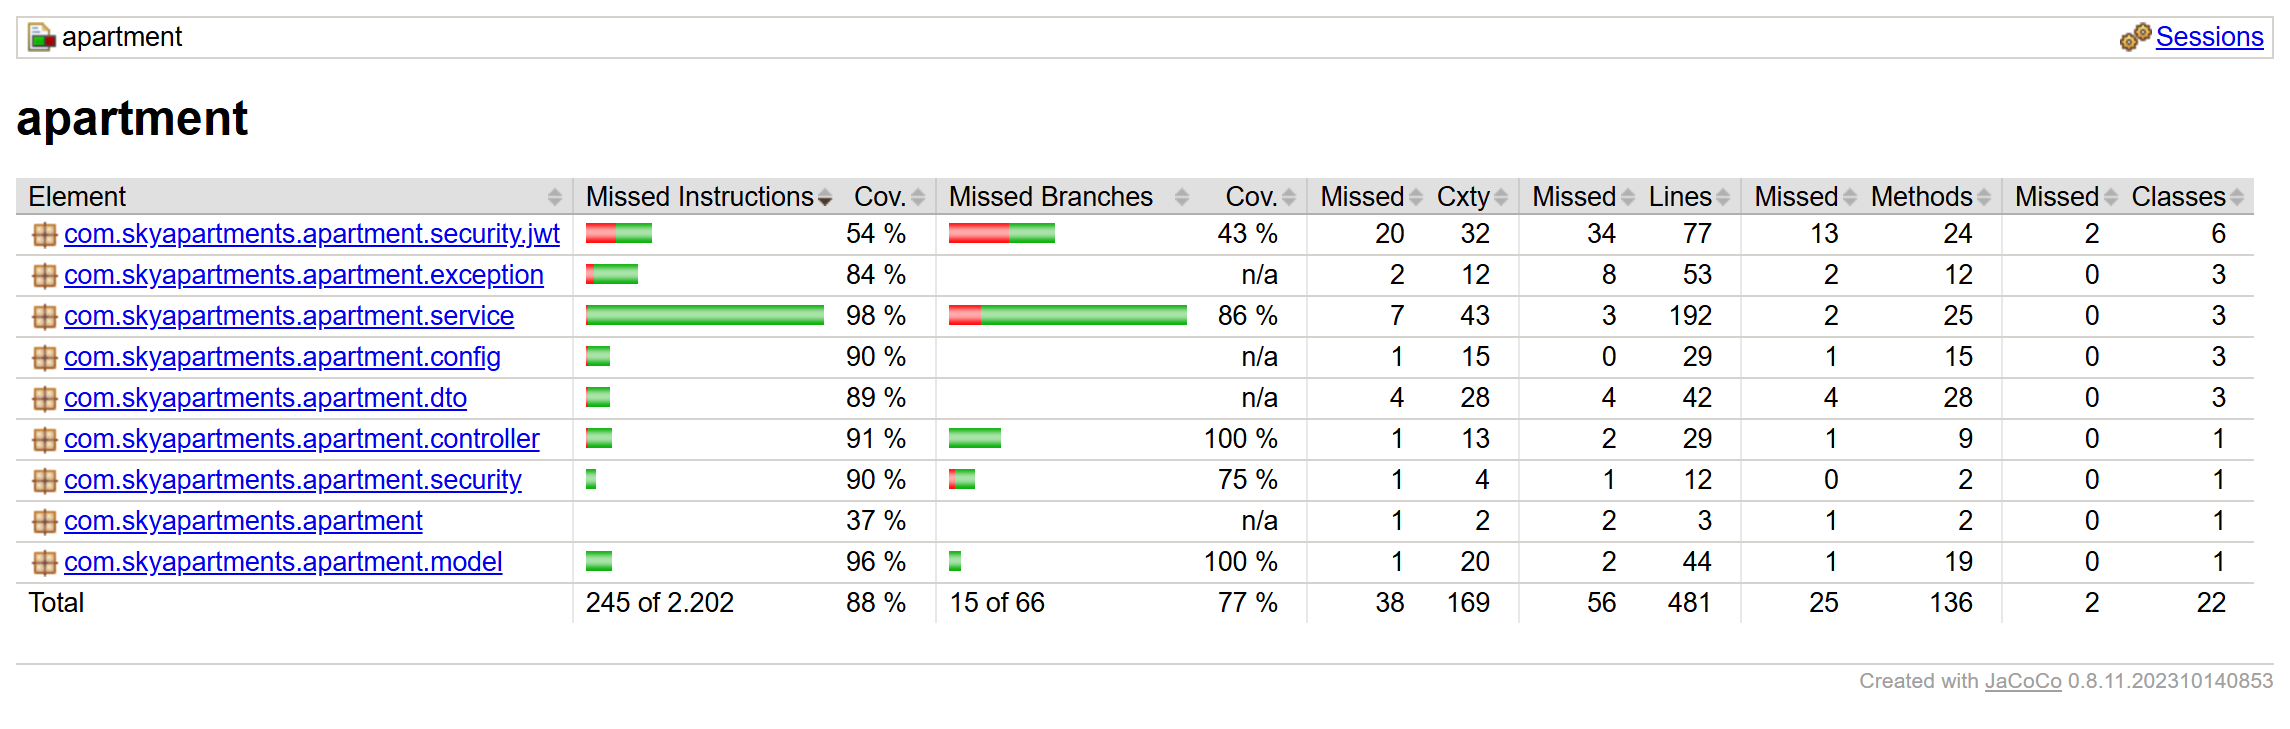
\includegraphics[width=0.9\textwidth]{img/jacoco_apartment.png}
\caption{Reporte de cobertura JaCoCo - Apartment Service}
\label{fig:jacoco_apartment}
\end{figure}

\begin{figure}[H]
\centering
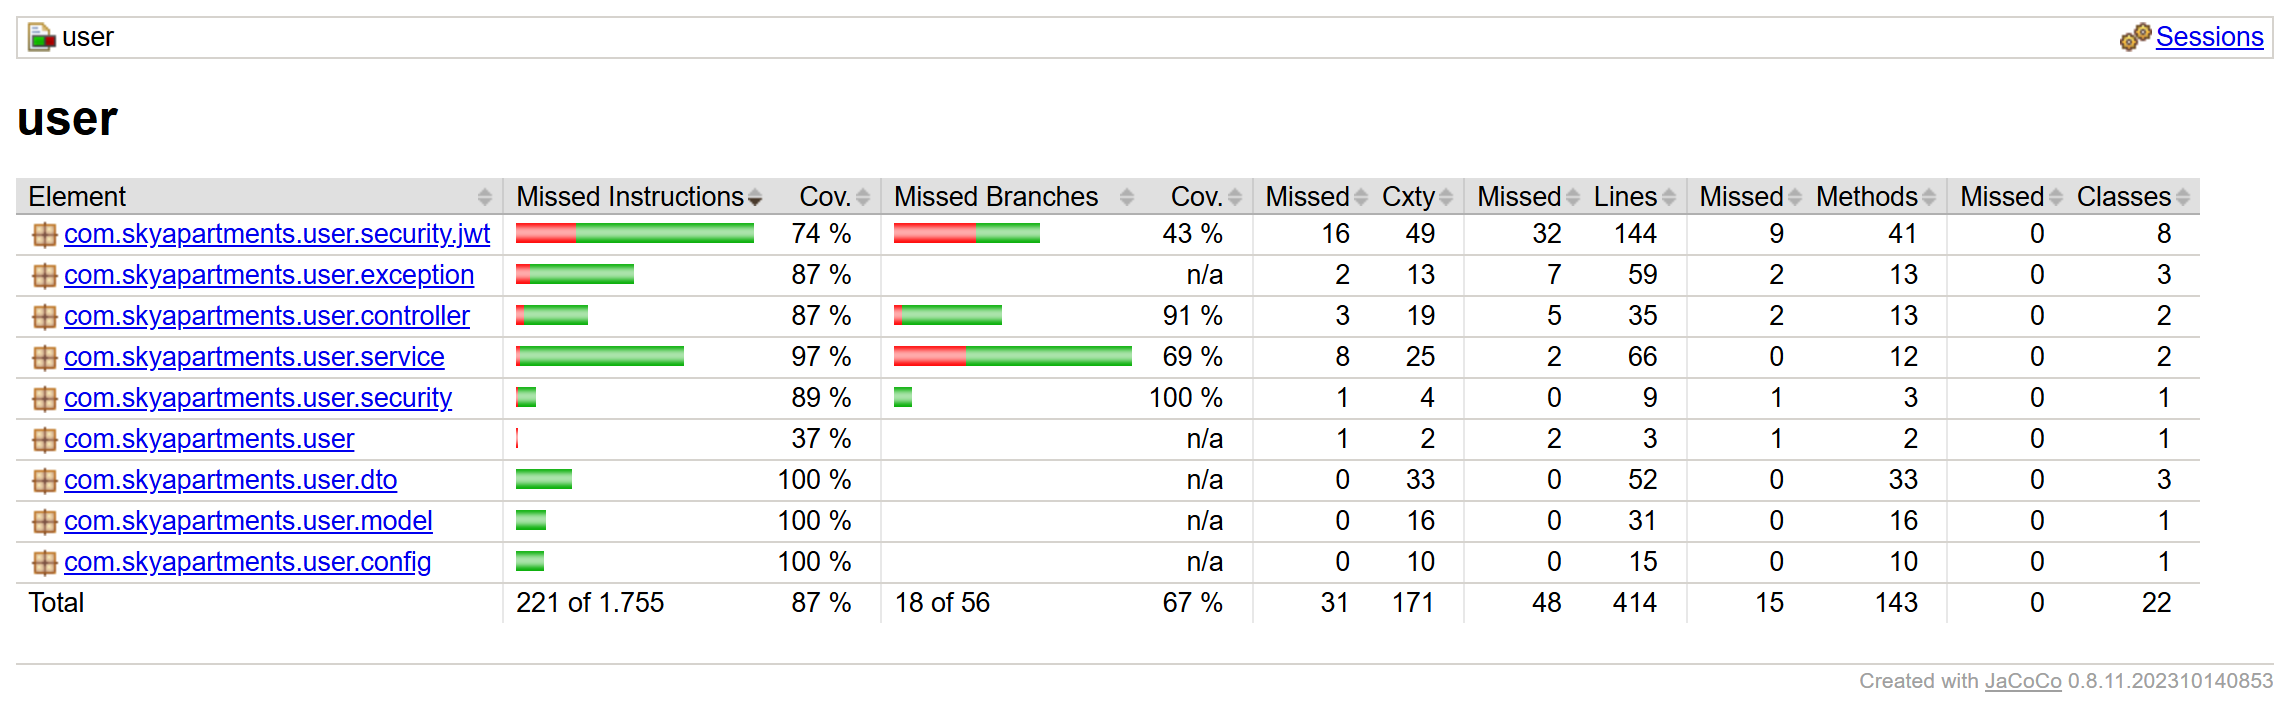
\includegraphics[width=0.9\textwidth]{img/jacoco_user.png}
\caption{Reporte de cobertura JaCoCo - User Service}
\label{fig:jacoco_user}
\end{figure}

\begin{figure}[H]
\centering
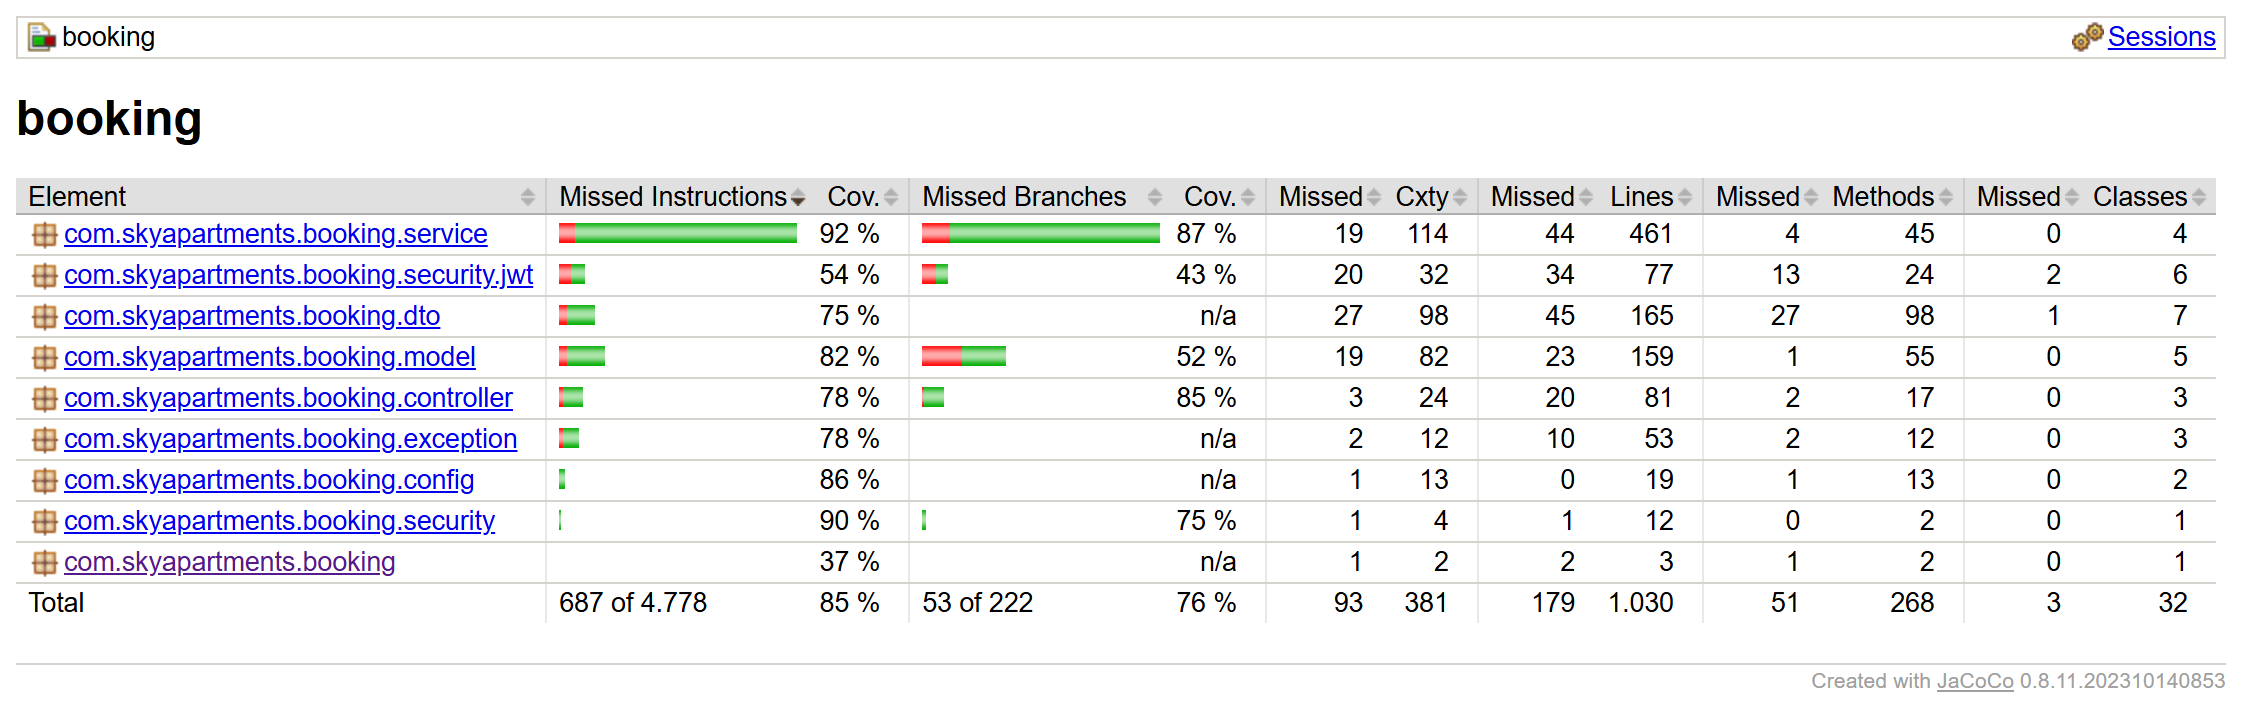
\includegraphics[width=0.9\textwidth]{img/jacoco_booking.png}
\caption{Reporte de cobertura JaCoCo - Booking Service}
\label{fig:jacoco_booking}
\end{figure}

\begin{figure}[H]
\centering
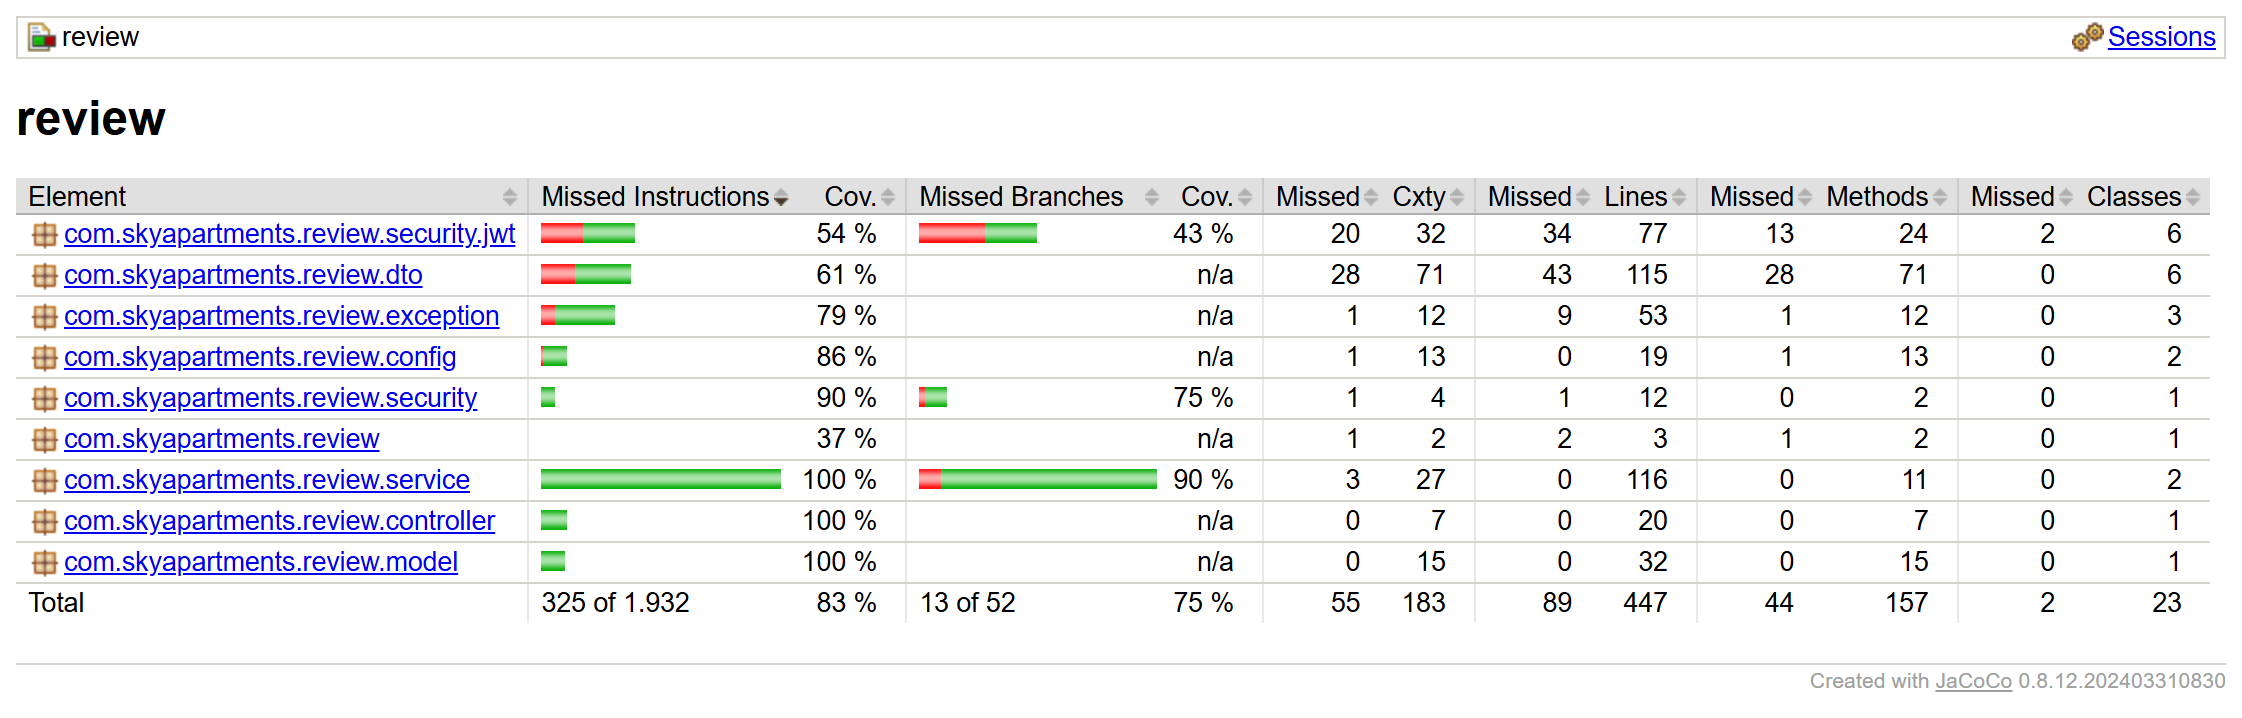
\includegraphics[width=0.9\textwidth]{img/jacoco_review.png}
\caption{Reporte de cobertura JaCoCo - Review Service}
\label{fig:jacoco_review}
\end{figure}

Los cuatro microservicios principales superan el umbral mínimo del 80\% de cobertura de líneas. Las capas de servicio y controladores alcanzan coberturas superiores al 75\% en todos los casos. Las entidades del modelo muestran coberturas del 82-100\% debido a que los tests de integración ejercitan exhaustivamente el mapeo JPA.

\subsection{Pruebas del frontend}
El frontend Angular ha sido testado en tres niveles: tests unitarios, tests de integración y tests end-to-end, garantizando tanto la corrección de componentes individuales como la validación de flujos completos de usuario.

\subsubsection{Tipos de Pruebas Implementadas}
\begin{itemize}
    \item \textbf{Tests Unitarios:} Validan la lógica de componentes aislados mediante un DOM virtual y servicios simulados (\textit{mocks}), empleando Jasmine como \textit{framework} y Karma como \textit{test runner}.
    \item \textbf{Tests de Integración:} Verifican la interacción entre componentes mediante \texttt{TestBed} de Angular, realizando peticiones HTTP reales al \textit{API Gateway} para validar el mapeo de objetos JSON y el manejo de errores.
    \item \textbf{Tests End-to-End (E2E):} Simulan flujos de usuario en navegadores reales mediante Playwright (clics, navegación, escritura). Requieren el backend en ejecución para certificar la integración completa entre el frontend y la base de datos.
\end{itemize}
\subsubsection{Cobertura de Tests Unitarios e Integración}
La cobertura del frontend se genera mediante Karma + Istanbul. El proyecto alcanza una cobertura del 90.94\% en líneas de código, 91.22\% en funciones, 82.34\% en ramas y 90.76\% en sentencias.

La Figura \ref{fig:frontend_coverage} muestra el reporte visual de cobertura generado por Istanbul, que permite identificar archivos con baja cobertura, líneas específicas no cubiertas, ramas condicionales no ejercitadas y funciones no invocadas durante los tests.

\begin{figure}[!h]
\centering
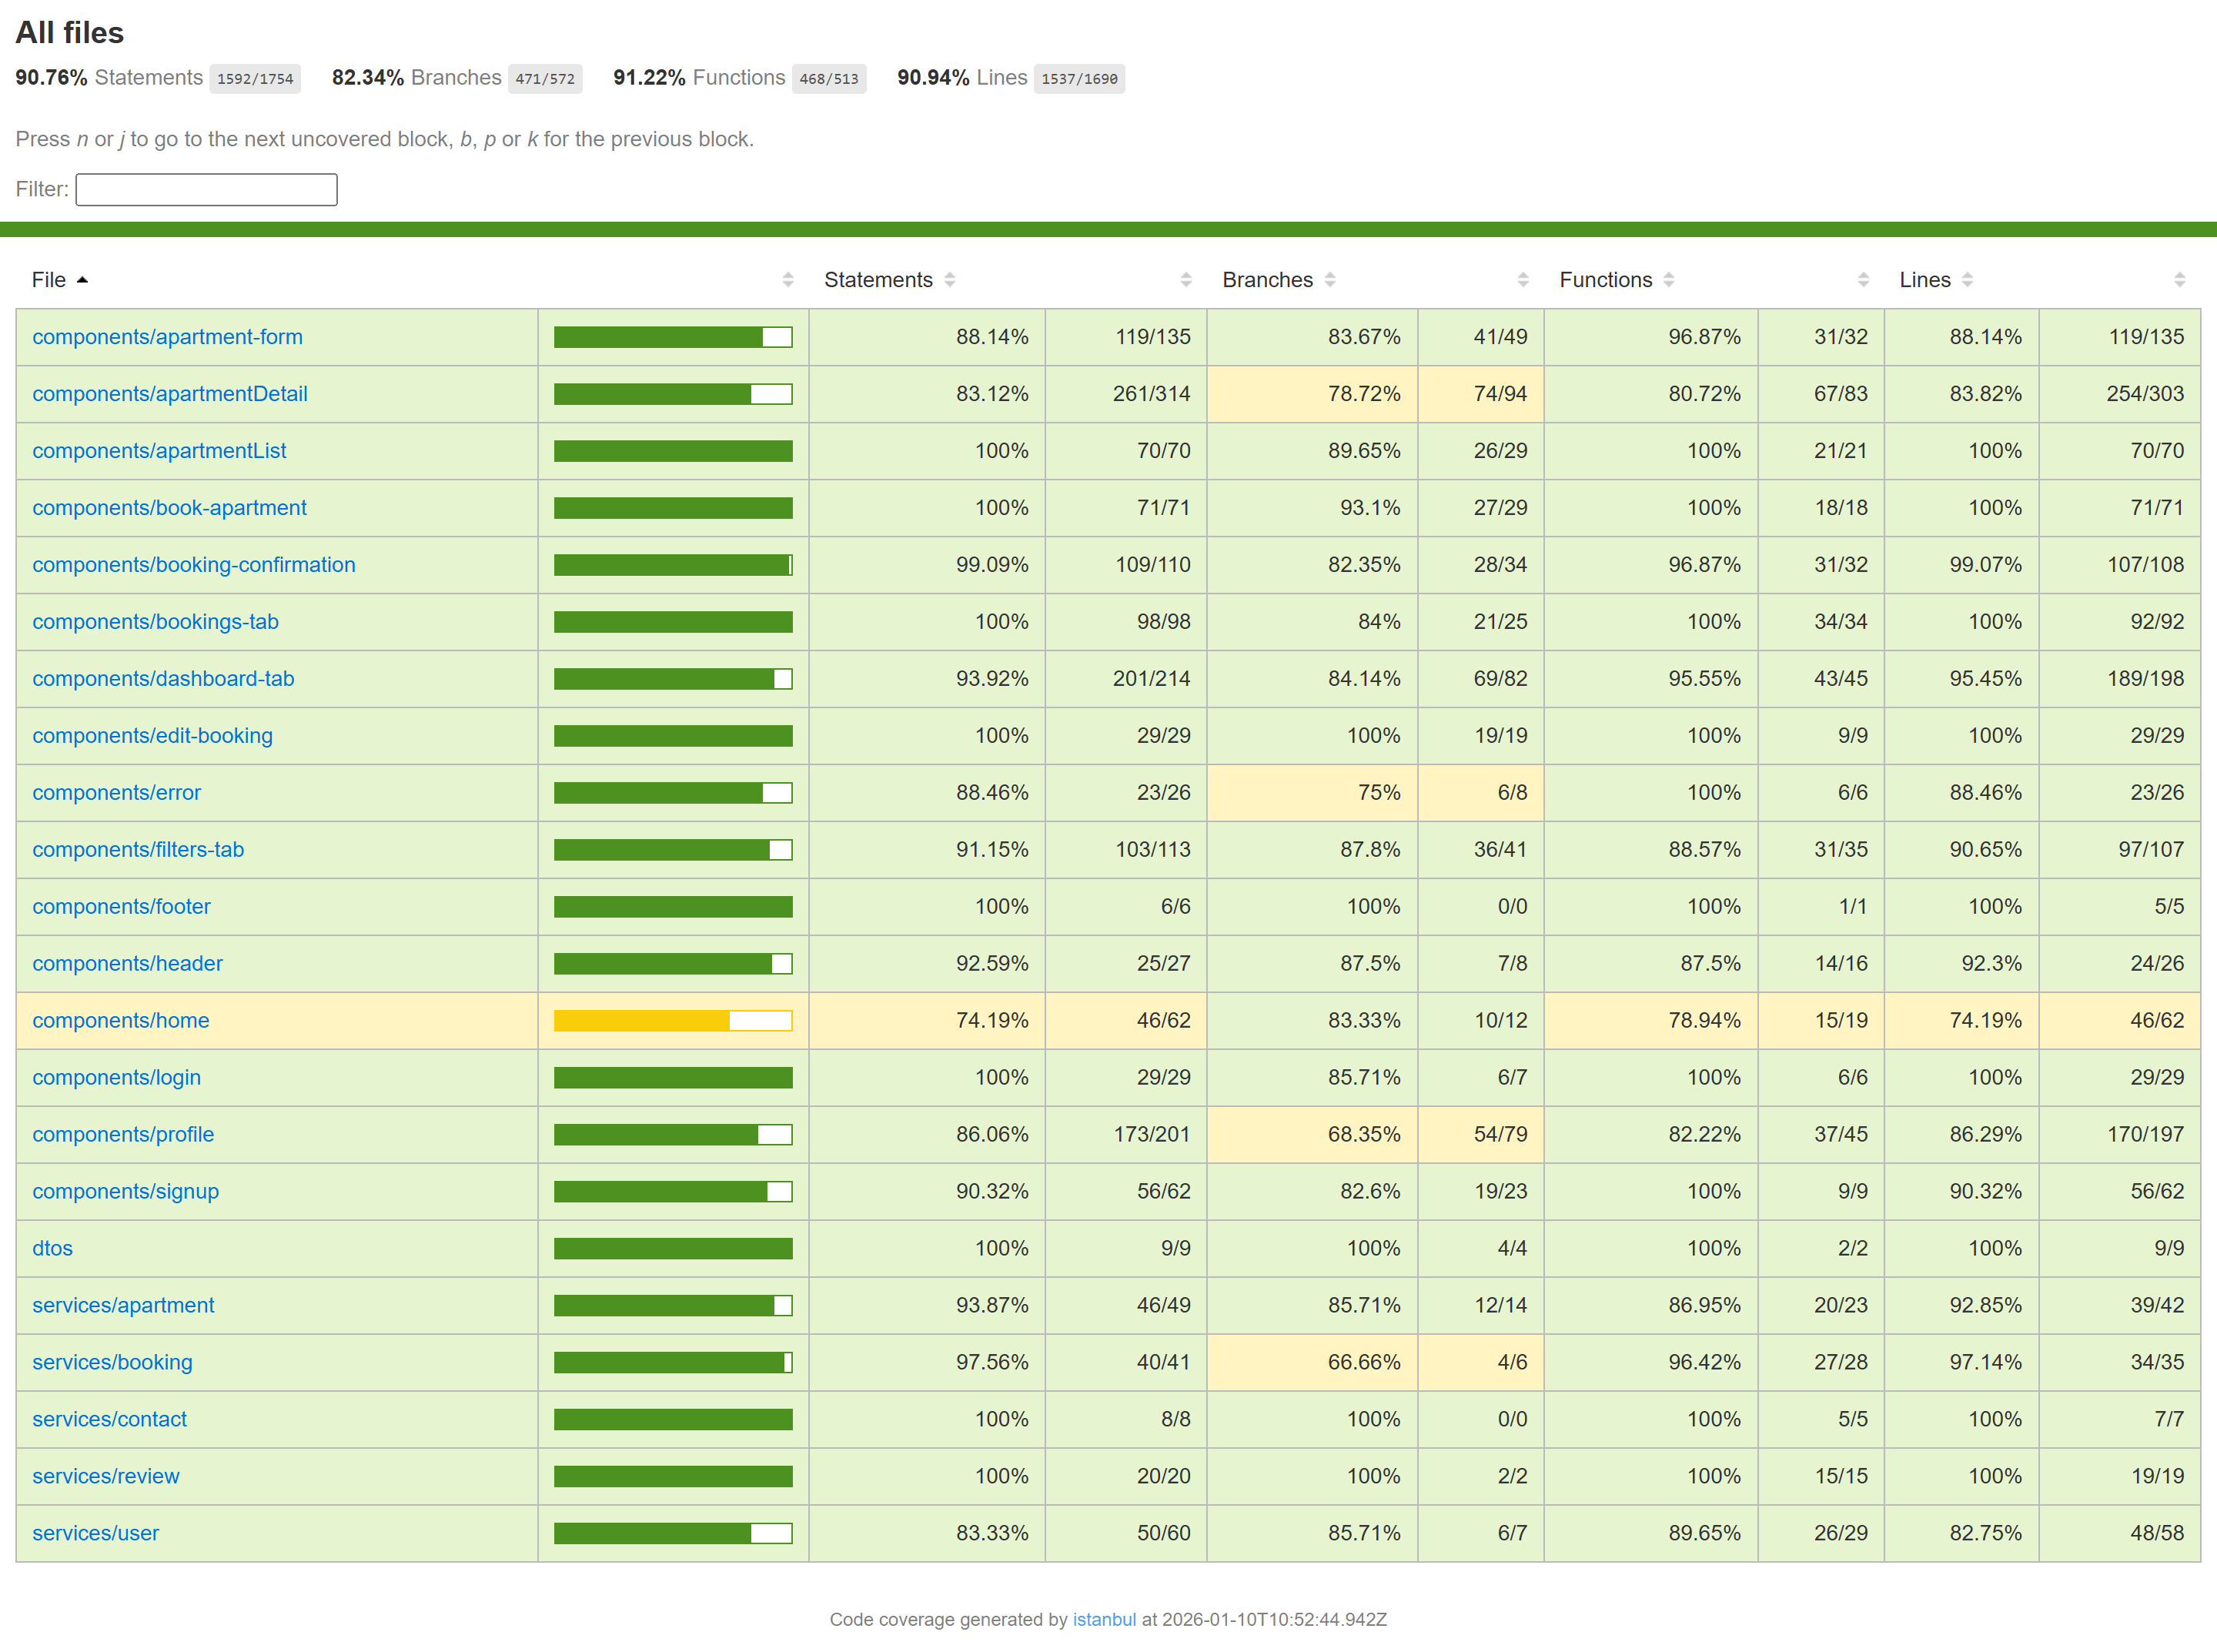
\includegraphics[width=0.95\textwidth]{img/informe_front.png}
\caption{Reporte de cobertura del frontend - Tests unitarios e integración}
\label{fig:frontend_coverage}
\end{figure}

\subsubsection{Tests End-to-End con Playwright}
Los tests E2E validan flujos completos incluyendo autenticación de usuarios, navegación y filtrado de apartamentos, creación y gestión de reservas, escritura de reseñas e interacciones que involucran múltiples microservicios.

\subsection{Análisis de Resultados}
El proyecto alcanza niveles de cobertura satisfactorios: 80-88\% de cobertura de líneas en el backend según el microservicio, 90.94\% en el frontend, y una cobertura global estimada de aproximadamente 85\% considerando todo el código del proyecto. Estos valores superan el umbral mínimo del 75-80\% considerado estándar en la industria, garantizando que la mayor parte del código está cubierta por tests automatizados que detectarían regresiones en futuras modificaciones.
\section{Despliegue}
\label{sec:despliegue}

En esta sección se describe el empaquetado mediante contenedores, la distribución de 
artefactos y el despliegue en la nube (AWS).

\subsection{Empaquetado y Distribución}

Para facilitar la distribución, se utiliza un \textit{Dockerfile multi-etapa} que genera 
\textbf{una única imagen Docker} agrupando el cliente (Angular) y el servidor (microservicios 
Spring Boot, Eureka y \textit{API Gateway}). Esta estrategia, adoptada por las limitaciones de recursos 
del entorno académico, garantiza un versionado coherente y optimiza el consumo de memoria de 
la instancia EC2. El proceso compila el backend (Maven/JDK 17) y el frontend (Node.js) de 
forma independiente, fusionando los binarios resultantes en una imagen final ligera 
(Alpine + JRE 17) orquestada por un \textit{script} de arranque secuencial.

Para gestionar el entorno completo se utiliza \textbf{Docker Compose}, inyectando la 
configuración sensible dinámicamente mediante un archivo \texttt{.env}. Este archivo define 
la infraestructura como código (\textit{Infrastructure as Code}), creando la red virtual, 
los volúmenes persistentes y coordinando:
\begin{itemize}
    \item El contenedor principal de la aplicación Sky Apartments.
    \item Un único motor \textbf{MySQL 8.0} con cuatro esquemas de base de datos independientes 
    (uno por microservicio: \texttt{usersdb}, \texttt{apartmentsdb}, \texttt{bookingsdb} y 
    \texttt{reviewsdb}), preservando el aislamiento lógico de datos que exige el patrón 
    \textit{Database per Service}~\cite[Cap.~5]{richardson2018}.
    \item MinIO (almacenamiento de objetos) y Jaeger (trazabilidad distribuida).
\end{itemize}

La imagen final y el manifiesto de infraestructura se distribuyen de forma pública a través 
de \textbf{DockerHub}, estando disponibles en la siguiente URL: \\
\url{https://hub.docker.com/r/eloydsdlh/apartments-app}

\subsection{Despliegue en la Nube (AWS)}

La aplicación está desplegada en producción sobre \textbf{Amazon Web Services (AWS)}, 
utilizando el servicio \textbf{Amazon EC2}. La Figura~\ref{fig:despliegue_aws} ilustra 
la topología de red del entorno de producción.

\begin{figure}[!h]
\centering
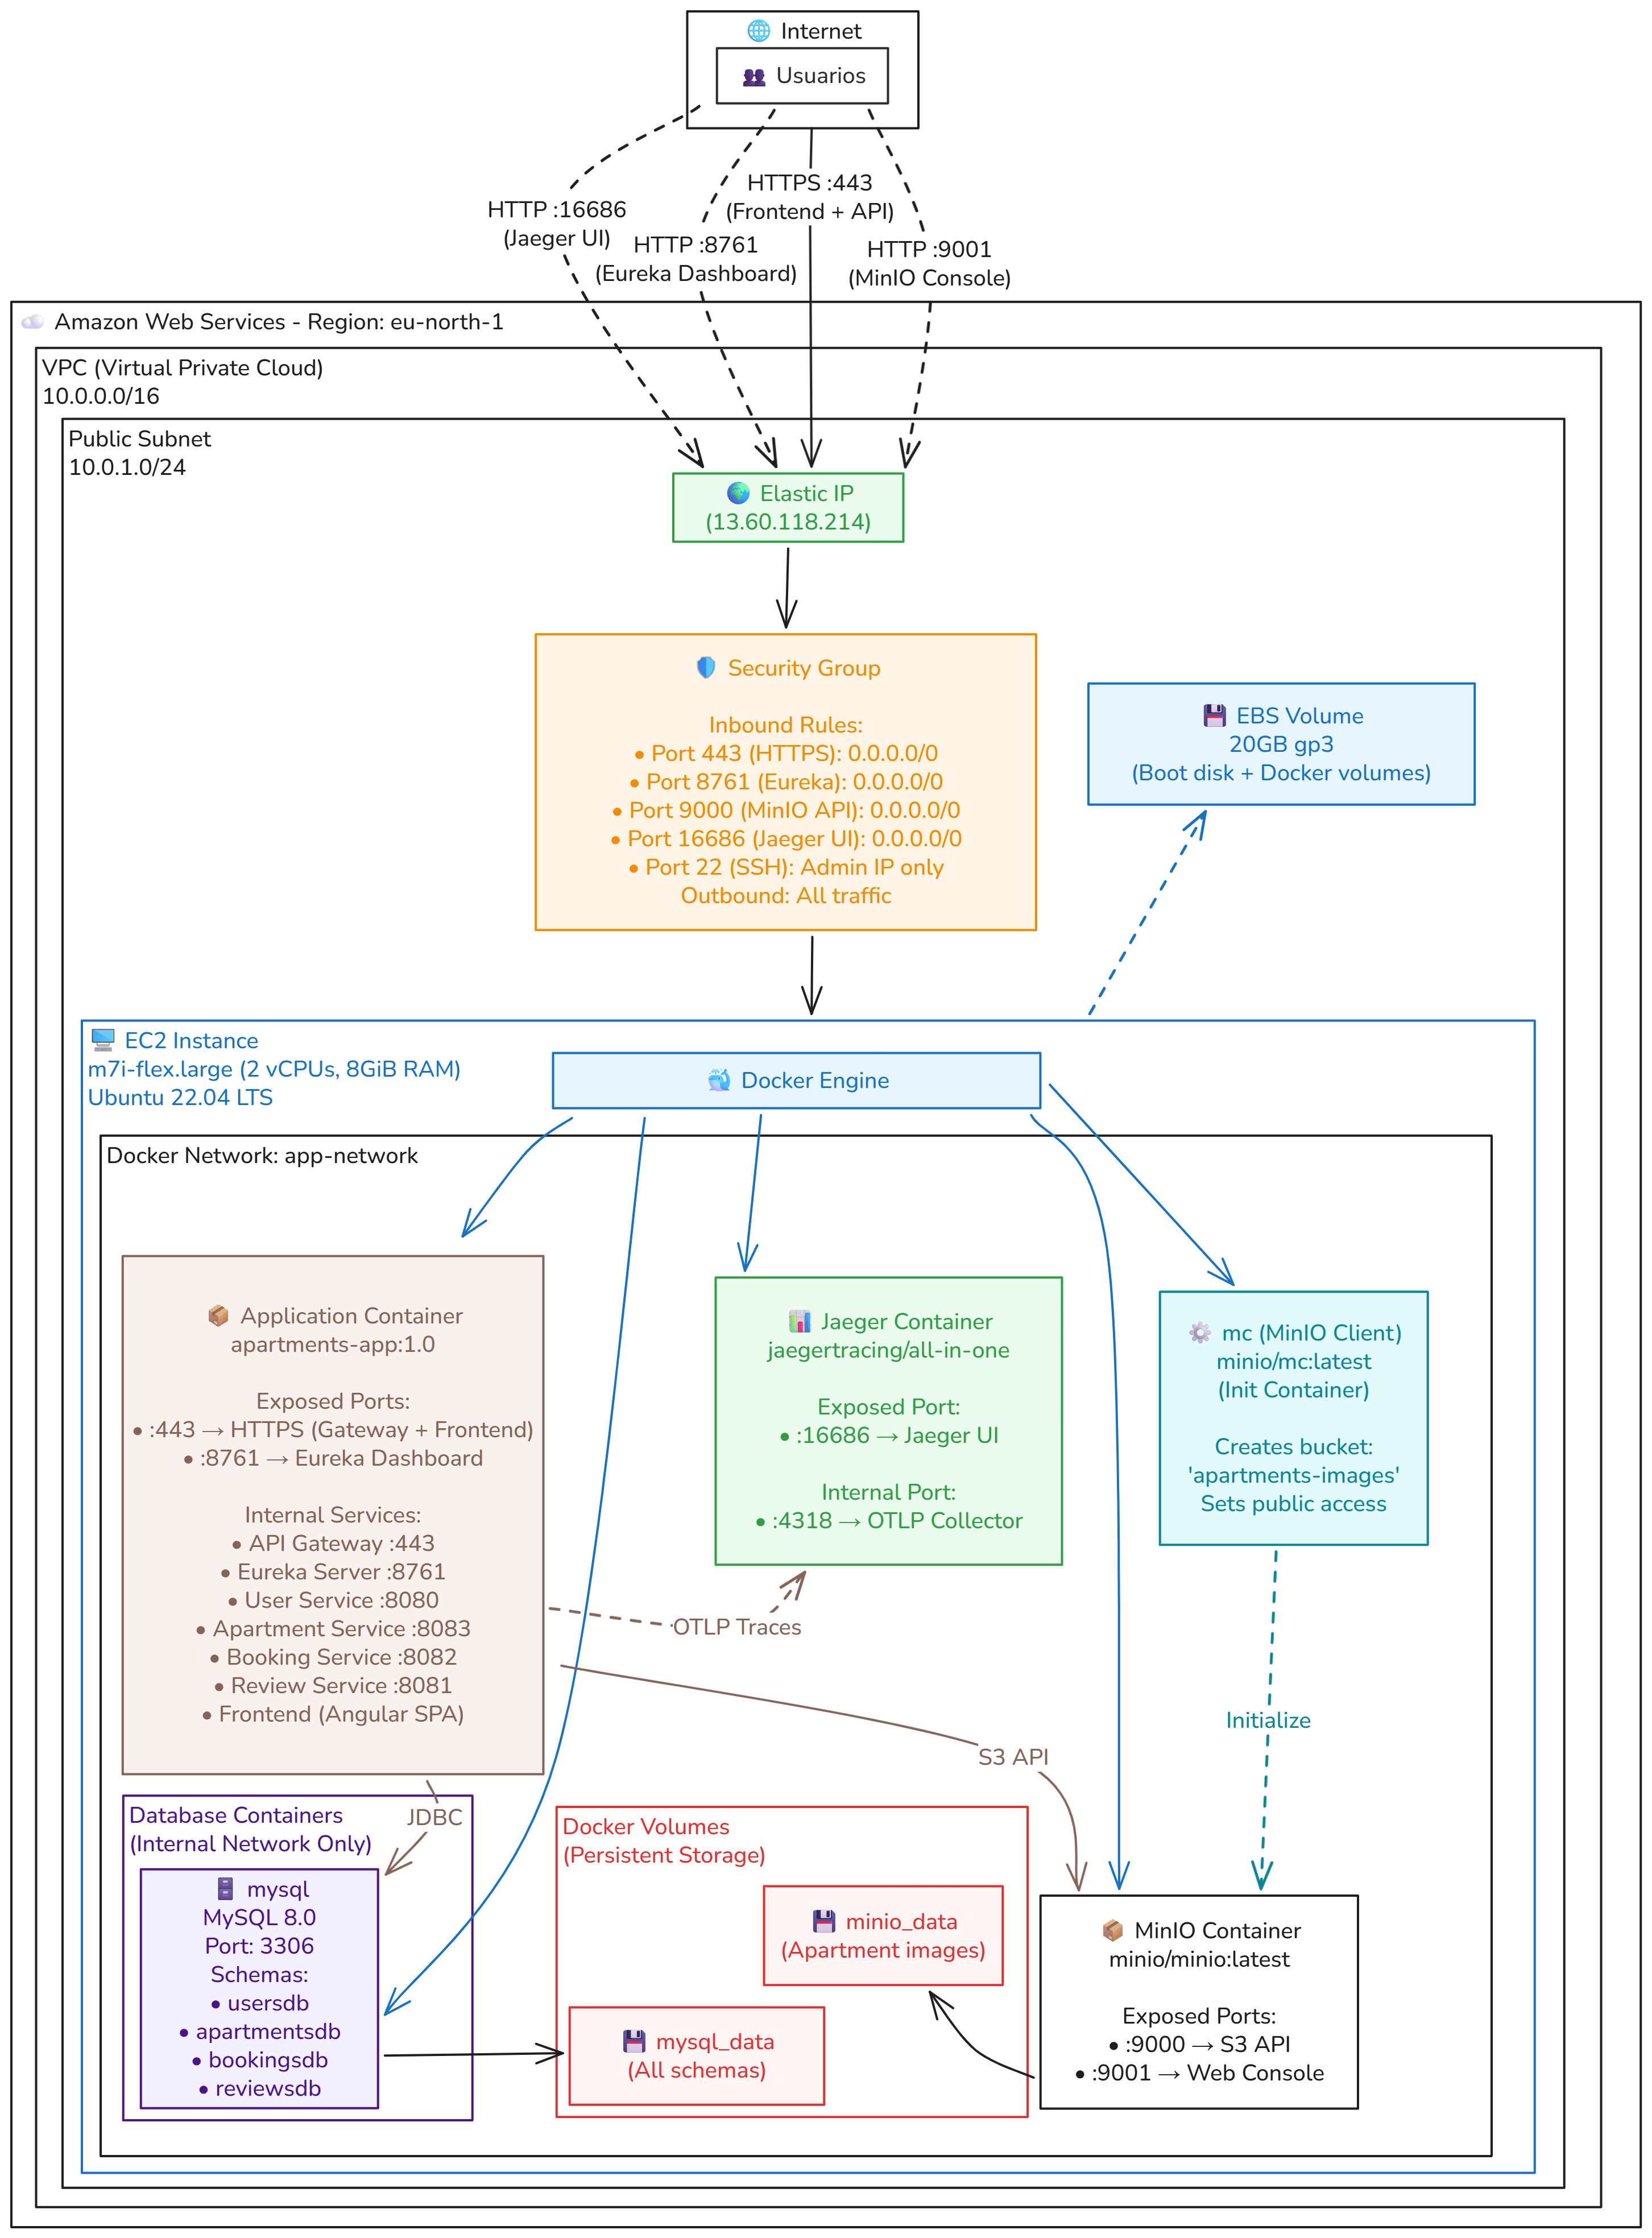
\includegraphics[width=\textwidth]{img/diagrama_despliegue.png}
\caption{Arquitectura de despliegue en Amazon EC2.}
\label{fig:despliegue_aws}
\end{figure}

\subsubsection{Arquitectura de Infraestructura}
La infraestructura consta de los siguientes componentes clave diseñados para garantizar 
el aislamiento y la seguridad:
\begin{itemize}
    \item \textbf{Instancia EC2 (m7i-flex.large):} Máquina con Ubuntu 22.04 LTS, 2 vCPUs 
    y 8 GiB de RAM para soportar las exigencias de memoria de la JVM.
    \item \textbf{Elastic IP:} Dirección IPv4 pública y estática (13.60.118.214).
    \item \textbf{Security Group (Firewall):} Expone el puerto 443 (HTTPS) al público, 
    reserva el 22 (SSH) para el administrador, y habilita los puertos 8761, 9001 y 16686 
    excepcionalmente para la evaluación académica del proyecto.
\end{itemize}

\subsubsection{Procedimiento de Despliegue}
El uso de artefactos OCI (\textit{Open Container Initiative}) hace que el despliegue sea 
altamente predecible y no requiera clonar el código fuente. Tras aprovisionar la máquina 
e instalar Docker, el administrador configura las credenciales y parámetros de 
infraestructura mediante un archivo de variables de entorno \texttt{.env}. El formato 
detallado de este archivo, así como la descripción de todas las variables disponibles, 
se detallan en el Anexo~\ref{anexo:instrucciones-ejecutar-aplicacion}.

Una vez configurado el entorno, se ejecuta un único comando que descarga el manifiesto 
directamente desde DockerHub:

\begin{verbatim}
docker compose -f oci://eloydsdlh/apartments-compose:1.0 up -d
\end{verbatim}

Este comando automatiza la descarga de imágenes, la creación de redes, la inicialización 
de los esquemas de base de datos y el inicio jerárquico dictado por los \textit{healthchecks} 
(levantando primero MySQL y MinIO antes que la aplicación principal). En cuestión de minutos, 
el orquestador registra los microservicios en Eureka y levanta el \textit{API Gateway}, dejando la 
aplicación operativa y accesible de forma segura.

\section{Proceso de Desarrollo} 
\label{sec:proceso_desarrollo}

El desarrollo se ha regido por un proceso \textbf{iterativo e incremental}, fuertemente alineado con los principios del Manifiesto Ágil ~\cite{ManifiestoAgil}. Se ha priorizado la entrega continua de valor, la adaptación al cambio y la automatización de procesos. Para ello, el proyecto se ha apoyado en prácticas fundamentales de la Programación Extrema (XP) ~\cite{Beck1999}, tales como la integración continua, el diseño guiado por pruebas automatizadas y las iteraciones cortas de desarrollo. 

La gestión del flujo de trabajo se ha fundamentado en metodologías visuales basadas en Kanban. Cabe destacar de manera explícita que no se ha aplicado el marco de trabajo Scrum, dado que sus ceremonias y artefactos no se adecúan a la naturaleza de un proyecto individual de esta índole.

\subsection{Gestión de Tareas} 
La planificación y el seguimiento del trabajo se han centralizado utilizando las herramientas nativas del repositorio: \textbf{GitHub Issues} y \textbf{GitHub Projects}. 

\begin{itemize}
    \item \textbf{GitHub Issues:} Se han utilizado como la unidad básica de trabajo, registrando en ellos los requisitos funcionales, la detección de errores (\textit{bugs}), mejoras técnicas y nuevas características.
    \item \textbf{GitHub Projects:} Ha proporcionado la capa de gestión visual. Mediante un tablero \textbf{Kanban}, los \textit{issues} se organizaron en columnas de estado (\textit{To Do}, \textit{In Progress}, \textit{Done}), permitiendo una priorización clara de las tareas y una monitorización en tiempo real del progreso del desarrollo. El tablero de gestión del proyecto es accesible en:
    \newline
    \url{https://github.com/orgs/codeurjc-students/projects/16}
\end{itemize}

Para analizar el progreso del proyecto a lo largo del tiempo, se ha utilizado un gráfico de \textit{Burn up} (Figura \ref{fig:burnup_chart}) extraído directamente de las analíticas del repositorio. Este gráfico ilustra la evolución del alcance del proyecto (tareas abiertas) frente a la velocidad de resolución (tareas completadas), evidenciando la naturaleza iterativa y adaptativa de la metodología empleada.

\begin{figure}[!h]
    \centering
    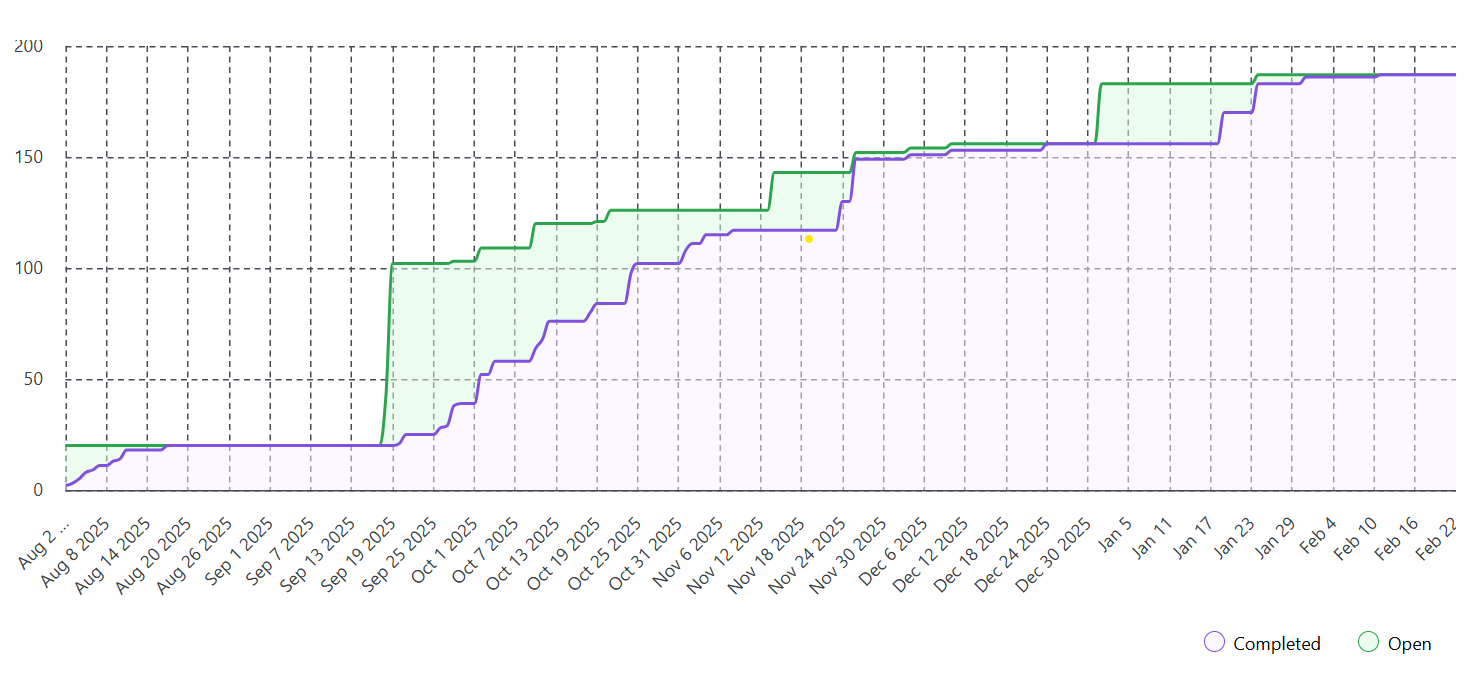
\includegraphics[width=\textwidth]{img/burnup_chart.png}
    \caption{Gráfico de Burn up del proyecto. La línea superior (verde) representa el total de tareas identificadas y la línea inferior (morada) las tareas completadas a lo largo del tiempo.}
    \label{fig:burnup_chart}
\end{figure}

\subsection{Control de Versiones con Git} 
El control de versiones del código fuente se ha gestionado íntegramente con \textbf{Git}, y el repositorio del proyecto se encuentra alojado públicamente en GitHub: \newline
\url{https://github.com/codeurjc-students/2025-sky-apartments}.\newline
Para garantizar la estabilidad del código, se ha implementado una estrategia de ramificación (\textit{branching strategy}) estricta basada en el modelo de \textit{feature branches}:

\begin{itemize}
    \item \textbf{Rama \texttt{main}:} Rama principal protegida. Contiene código estable y siempre listo para ser desplegado.
    \item \textbf{Ramas de característica (\texttt{feature/*}):} Creadas a partir de \texttt{main} para desarrollar de forma aislada cada nueva funcionalidad.
    \item \textbf{Ramas de corrección (\texttt{fix/*}):} Destinadas exclusivamente a la resolución de errores detectados.
    \item \textbf{Ramas auxiliares (\texttt{testing/*}, \texttt{ci/*}, \texttt{docs/*}):} Utilizadas para la configuración de flujos de trabajo, pruebas de integración continua y redacción de documentación.
\end{itemize}

La integración de código hacia la rama \texttt{main} se ha realizado exclusivamente mediante \textbf{Pull Requests} (PR), forzando la revisión de código y la ejecución de los flujos de integración continua antes de permitir la fusión. 

A la fecha de cierre de este documento, el repositorio cuenta con un histórico sólido y altamente estructurado, registrando un total de \textbf{346 \textit{commits}}, \textbf{67 ramas} creadas para aislar el trabajo y \textbf{63 \textit{Pull Requests}}.

\subsection{Integración y Entrega Continua (CI)} 
La automatización de la calidad del código se ha orquestado mediante \textbf{GitHub Actions}, definiendo múltiples flujos de trabajo que actúan como barreras de calidad en diferentes etapas.
\subsubsection{Basic Quality Check}
Se ejecuta con cada (\textit{push}) a las ramas de desarrollo. Su objetivo es proporcionar retroalimentación rápida al desarrollador:
\begin{itemize}
    \item \textbf{\texttt{backend-basic}:} Ejecuta las pruebas unitarias aisladas para todos los microservicios Java (Apartment, User, Booking, Review).
    \item \textbf{\texttt{frontend-basic}:} Instala dependencias y ejecuta la suite de pruebas unitarias de Angular.
\end{itemize}

\subsubsection{Full Quality Check}
Se activa al abrir o actualizar una \textit{Pull Request} hacia la rama \texttt{main}. Es un flujo exhaustivo y secuencial que levanta toda la infraestructura para validar el sistema en su conjunto:
\begin{enumerate}
    \item \textbf{\texttt{backend-unit-integration}:} Ejecuta pruebas unitarias y de integración del backend, utilizando \textbf{Testcontainers} para levantar bases de datos MySQL efímeras.
    \item \textbf{\texttt{backend-e2e}:} Tras compilar los microservicios, utiliza Docker Compose para levantar la infraestructura completa (Bases de datos, MinIO, Eureka, Gateway, Jaeger y microservicios). Valida la comunicación cruzada entre servicios ejecutando pruebas End-to-End en el backend, esperando a que todos los servicios se registren sanos en Eureka.
    \item \textbf{\texttt{frontend-integration}:} Ejecuta pruebas de integración en el cliente web conectándose a los microservicios levantados en el paso anterior a través del \textit{API Gateway}.
    \item \textbf{\texttt{frontend-e2e}:} Instala los navegadores de \textbf{Playwright}, arranca el servidor de desarrollo de Angular y simula interacciones reales de usuario, validando flujos completos desde la interfaz gráfica hasta la base de datos.
    \item \textbf{\texttt{frontend-unit}:} Ejecuta la suite de pruebas unitarias del cliente web mediante Karma y Jasmine para validar la lógica aislada.
\end{enumerate}

Toda esta infraestructura efímera inyecta las variables de entorno mediante los \textit{Secrets} de GitHub de forma segura y destruye los contenedores tras finalizar las pruebas, garantizando un entorno limpio en cada ejecución.

\subsection{Entrega Continua y Versionado} 
El proyecto emplea un sistema de \textbf{entrega continua} automatizado mediante GitHub Actions para publicar las imágenes en DockerHub. El paso a producción (AWS) se realiza de forma manual y controlada, rigiéndose por un \textbf{versionado semántico} gestionado a través de \textit{Releases} de GitHub.

\subsubsection{Gestión de Versiones y Publicación}
Los \textit{merges} en \texttt{main} generan automáticamente la imagen \texttt{:dev}, mientras que al crear una \textit{Release} se sincronizan las versiones internas (\texttt{pom.xml}, \texttt{package.json}) y se publican las imágenes definitivas etiquetadas con su versión (ej. \texttt{:0.1}) y como \texttt{:latest}.


\subsubsection{Historial de Lanzamientos}
A lo largo del proyecto se han publicado tres iteraciones mayores:
\begin{itemize}
    \item \textbf{08/11/2025 -- v0.1 (MVP Técnico):} Cimientos arquitectónicos, seguridad (HTTPS), despliegue inicial con Docker y CRUD básico de usuarios, apartamentos y reservas.
    \item \textbf{24/12/2025 -- v0.2 (UX y Cloud):} Despliegue oficial en AWS EC2. Integró galerías (MinIO), calendarios en tiempo real, emails automatizados, reseñas y el \textit{Dashboard} administrativo.
    \item \textbf{01/02/2026 -- v1.0 (Lógica Avanzada):} Versión final. Introdujo el motor de precios dinámicos, recordatorios automáticos de \textit{check-in} y filtrado avanzado.
\end{itemize}

\subsubsection{Impacto en los usuarios durante el despliegue}
El despliegue sobre Amazon EC2 conlleva un breve \textit{downtime} planificado: el administrador ejecuta \texttt{docker compose down} y \texttt{docker compose up -d} para descargar las nuevas imágenes e iniciar los servicios. Esta sustitución directa, aunque implica unos minutos de inactividad, es adecuada para la escala académica del proyecto.